\documentclass[8pt,xcolor=table]{beamer}

\usepackage{graphicx}
\usepackage{caption}
\usepackage{subcaption}
 
% \usepackage[utf8]{inputenc}
% \usepackage[T1]{fontenc}
\usepackage[table]{xcolor}    % loads also »colortbl« 
%  \usepackage{enumitem}
\usepackage{ucltemplate}
\usepackage{color}

\usepackage{pgfgantt} % for grantt charts
\usepackage{rotating}
\usepackage[graphicx]{realboxes}
\usepackage[export]{adjustbox}
\usepackage{array,booktabs}

\usepackage{rotating}
% \usepackage{tabularx, booktabs} % make width of table columns evenly distributed (see http://tex.stackexchange.com/questions/60601/evenly-distributing-column-widths)
% \newcolumntype{Y}{>{\centering\arraybackslash}X}


\DeclareMathOperator*{\argmin}{arg\,min}
\DeclareMathOperator*{\argmax}{arg\,max}

\usepackage{tikz}
\usetikzlibrary{arrows,positioning, shapes.symbols,shapes.callouts,patterns,shapes,chains,calc,backgrounds,fadings}

% \definecolor{parCol}{rgb}{0.1, 0.1, 1}
% \definecolor{stCol}{rgb}{0.1, 0.6, 0.1}
% \definecolor{bothCol}{rgb}{0, 0.5, 0.5}

\definecolor{parCol}{rgb}{0, 0, 0}
\definecolor{stCol}{rgb}{0, 0, 0}
\definecolor{bothCol}{rgb}{0, 0, 0}
 
%Information to be included in the title page:
\title{A vertex clustering model of disease progression}
\author{R. V. Marinescu\inst{1}, A. Eshaghi\inst{1,2}, 
M. Lorenzi\inst{1,4}, A. L. Young\inst{1}, N. P. Oxtoby\inst{1}, \\S. Garbarino\inst{1}, T. J. Shakespeare\inst{3}, S. J. Crutch\inst{3} and D. C. Alexander\inst{1}}

\institute{\small{\textsuperscript{1}Centre for Medical Image Computing, University College London, UK}

\textsuperscript{2}Queen Square MS Centre, UCL Institute of Neurology, London

\textsuperscript{3}Dementia Research Centre, UCL Institute of Neurology, University College London, UK

\textsuperscript{4}University of C\^{o}te d'Azur, Inria Sophia Antipolis, Asclepios Research Project
\vspace{0em}
}
\date{}

% logo of my university
\titlegraphic{
   \begin{figure}
   \begin{subfigure}{0.32\textwidth}
   \hspace{2em}
   
\includegraphics[height=1.0cm]{epsrc_logo.jpg}
   \end{subfigure}
   \begin{subfigure}{0.32\textwidth}
   \centering
   
\includegraphics[height=1.5cm]{NEWpond2017b.png} 
   \end{subfigure}
   \begin{subfigure}{0.32\textwidth}
   \centering
   
\includegraphics[height=1.0cm]{pondLogo.png} 
   \end{subfigure}
   \end{figure}
}

\setbeamercolor{frametitle}{fg=white}
\setbeamercolor{author in head/foot}{fg=white, bg=black} 
\setbeamercolor{institute in head/foot}{fg=white, bg=black} 
\setbeamercolor{title in head/foot}{fg=white, bg=black}
\setbeamercolor{date in head/foot}{fg=white, bg=black}

\setbeamersize{text margin left=10pt,text margin right=10pt}
\setbeamertemplate{frametitle}{
    \vspace{0.9em}
    \insertframetitle
%     \vspace{-3em}
}
\setbeamertemplate{footline}
{
  \vspace{-3em}
  \leavevmode%
  \hbox{%
  \begin{beamercolorbox}[wd=.25\paperwidth,ht=2.25ex,dp=1ex,center]{author in head/foot}%
    \usebeamerfont{author in head/foot}Razvan V. Marinescu
  \end{beamercolorbox}%
  \begin{beamercolorbox}[wd=.25\paperwidth,ht=2.25ex,dp=1ex,center]{institute in head/foot}%
    \usebeamerfont{institute in head/foot}University College London
  \end{beamercolorbox}%
  \begin{beamercolorbox}[wd=.25\paperwidth,ht=2.25ex,dp=1ex,center]{title in head/foot}%
    \usebeamerfont{title in head/foot}\insertsection
  \end{beamercolorbox}%
  \begin{beamercolorbox}[wd=.25\paperwidth,ht=2.25ex,dp=1ex,right]{date in head/foot}%
    \usebeamerfont{date in head/foot}\insertshortdate{}\hspace*{2em}
    \insertframenumber{} / \inserttotalframenumber\hspace*{2ex} 
  \end{beamercolorbox}}%
  \vskip0pt%
}
\makeatother
\beamertemplatenavigationsymbolsempty
\setbeamertemplate{caption}[numbered]
\setbeamercolor{caption name}{fg=black}
\setbeamercolor{itemize item}{fg=black}
\setbeamercolor{itemize subitem}{fg=black}
\setbeamercolor{enumerate item}{fg=black}
\setbeamercolor{enumerate subitem}{fg=black}
\setbeamertemplate{enumerate item}[default]
\setbeamertemplate{enumerate subitem}[default]
\begin{document}
 
\section{Introduction}

\frame{\titlepage}
 
\setbeamerfont{frametitle}{size=\large}

\newcommand{\imgFold}{../../../upgrade_report/images/vwdpm}


\begin{frame}
\frametitle{Aim}

\textbf{Aim}: Build a disease progression model of pathology over the brain that:

\newcommand{\aimImgScale}{0.8}
\newcommand{\mnpHeight}{3cm}

% FWHM0 avg thickness map MCI & AD
\begin{figure}[h]
  \centering
  \begin{minipage}[t][\mnpHeight][t]{0.3\textwidth}
   \centering
   Avoids pre-defined ROI parcellation\\
  \begin{tikzpicture}[scale=1]
    \node[inner sep=0] (image) at (0,0) {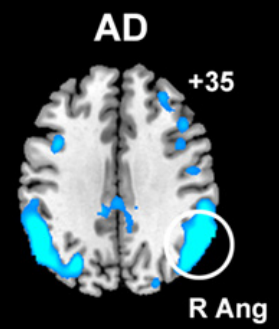
\includegraphics[width=0.5\textwidth,trim=0 0 26 0,clip]{seeley_2009_topleft.png}}; 
  \end{tikzpicture}
%     \caption{}
%       \label{fig:adniClust}
  \end{minipage}
   \begin{minipage}[t][\mnpHeight][t]{0.3\textwidth}
  \centering
  Avoids simplistic spatial correlation structure\\
%   \vspace{1em}
  \begin{tikzpicture}[scale=1]
    \node[inner sep=0] (corr_text) at (0,0) {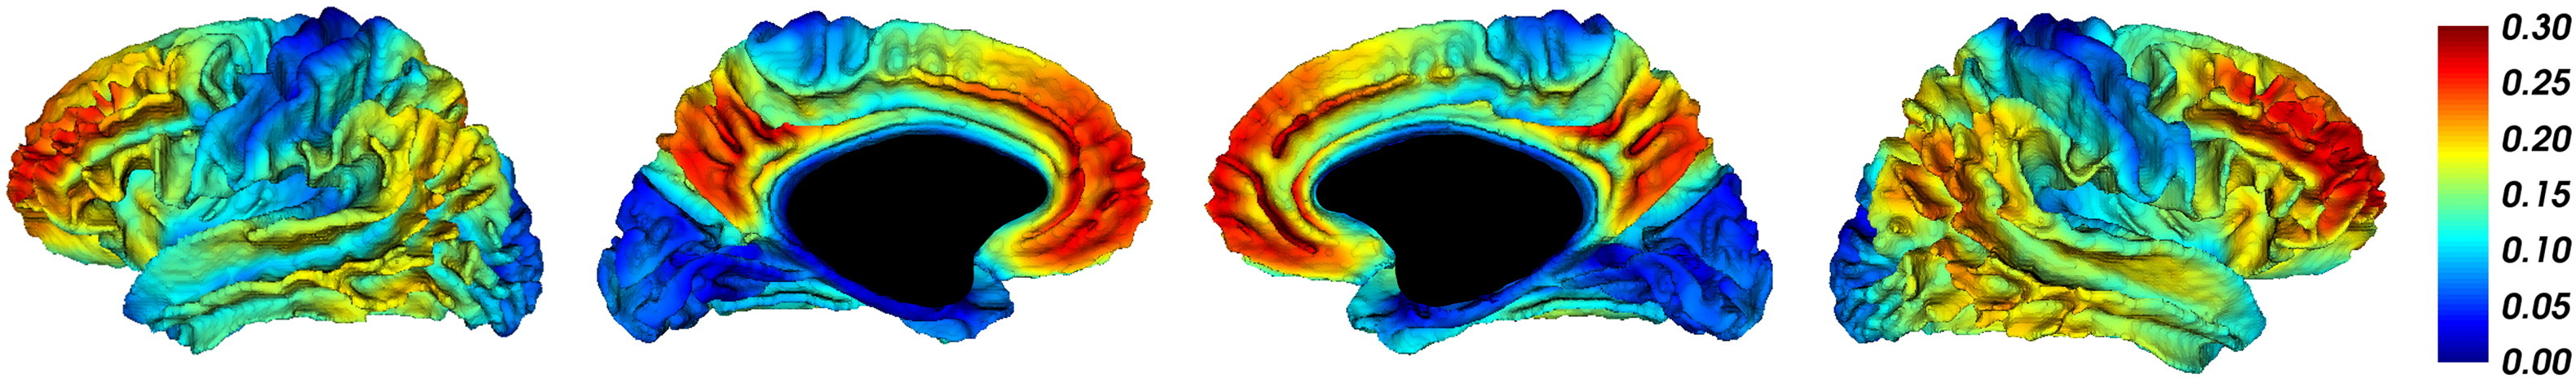
\includegraphics[width=\aimImgScale\textwidth, trim=0 0 360 0, clip]{bilgel_neuroimage}};
  \end{tikzpicture}
  \vspace{0.5em}
  \end{minipage}
   \begin{minipage}[t][\mnpHeight][t]{0.3\textwidth}
  \centering
  Avoids simplistic biomarker trajectories
  \begin{tikzpicture}[scale=1]
    \node[inner sep=0] (corr_text) at (0,0) {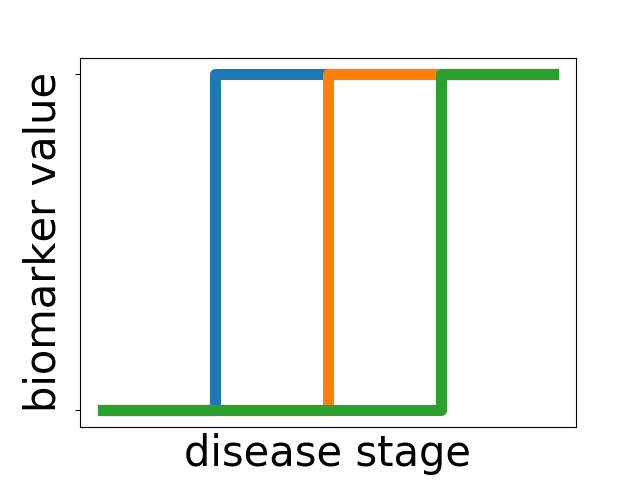
\includegraphics[width=\aimImgScale\textwidth,trim=0 0 0 30,clip]{biomkStepFunctions}};
  \end{tikzpicture}
  \end{minipage}
\end{figure}

\vfill

This leads to a technique that simultaneously:
\begin{itemize}
 \item parcellates the brain into disconnected components that undergo similar progression
 \item estimates biomarker trajectories
\end{itemize}


\end{frame}


\begin{frame}
\frametitle{Motivation}

\textbf{Aim}: Move from ROI-based analysis to vertexwise:
\begin{figure}
 \centering
  \begin{tikzpicture}[scale=1]
     \node (roi) at (0,0) {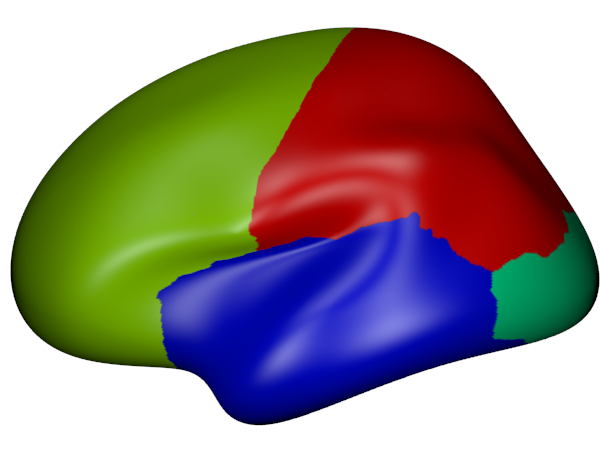
\includegraphics[scale=0.10]{clust24_drcThFWHM0InitfsurfCl4Pr0Ra1Mrf5_VWDPMStaticPCA.png}};
     \node (vw) at (4,0) {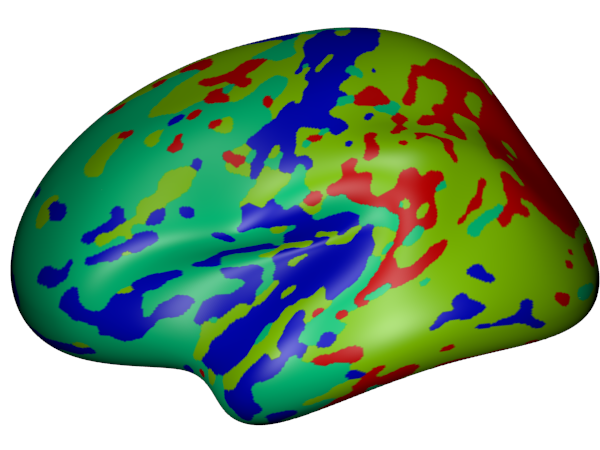
\includegraphics[scale=0.10]{clust24_drcThFWHM0Initk-meansCl4Pr0Ra1Mrf5_VDPM_MRFPCA.png}};
     \draw[line width=1.5,->] (roi) -> (vw);
  \end{tikzpicture}
\end{figure}

% \vfill

\begin{figure}
\begin{subfigure}{0.48\textwidth}
\textbf{Motivation}:
\begin{enumerate}
\item Atrophy correlates with functional networks, which are not spatially connected (Seeley et al., Neuron, 2009)
\vspace{2em}
\item Better biomarker prediction and disease staging
\end{enumerate}
\end{subfigure}
% \hspace{1em}
\begin{subfigure}{0.5\textwidth}
\centering 
% \vspace{-5em}
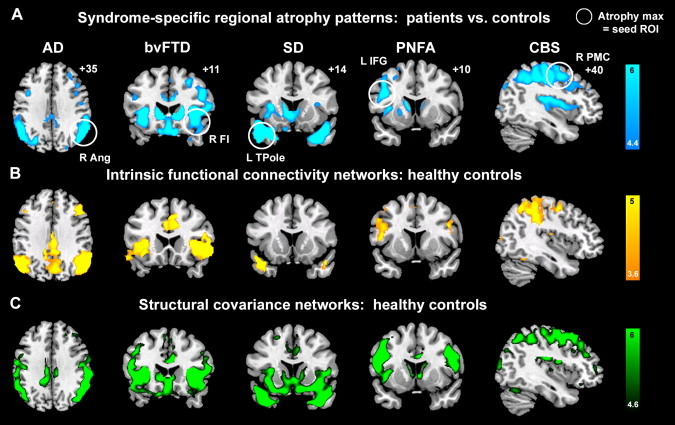
\includegraphics[width=\textwidth, right, trim=0 85 0 0, clip]{seeley_connectivity_overlap.jpg}
\caption{Seeley et al., Neuron, 2009}
\end{subfigure}

\end{figure}

\vfill

\vspace{-3em}


\end{frame}

%%%%%%%%%%%%%%%%%%%%%%%%%%%%%%%%%%%%%%%%%%%%


\begin{frame}
\frametitle{Background - Disease Progression Modelling}

\newcommand{\mnpHeight}{3cm}

\vspace{-3em}
% \textbf{Background}:
\begin{itemize}
  \item Modelling the progression of Alzheimer's disease can potentially help drug development
  \item Several data-driven disease progression models have been recently formulated:
  
%   \vfill 
  
  \hspace{-2em}
  \begin{small}
  \begin{figure}[h]
  \centering
    \begin{minipage}[t][\mnpHeight][t]{0.49\linewidth}
   \centering
    \textbf{Event-Based Model}\\ \footnotesize{(Fontejin et al., Neuroimage, 2012, Young et al., Brain, 2014)}\\    %TODO fix alignment of brains here
    \begin{subfigure}{0.57\textwidth}
    \vspace{-9em}
    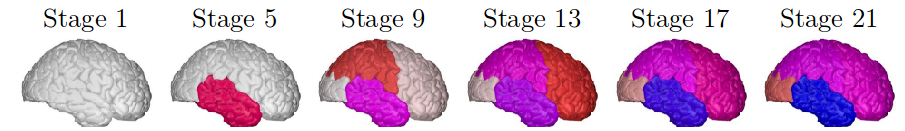
\includegraphics[width=\textwidth,trim=0 0 450 0,clip]{young_progression2}
    
    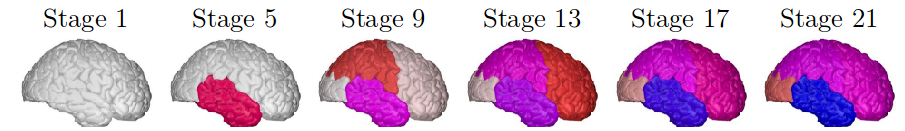
\includegraphics[width=\textwidth,trim=450 0 0 0,clip]{young_progression2} 
    \end{subfigure}
%     \vspace{1em}
    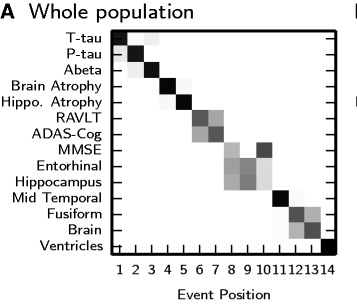
\includegraphics[width=0.4\textwidth]{young_positional_variance}
   \end{minipage}
   \begin{minipage}[t][\mnpHeight][t]{0.49\linewidth}
    \centering
    \textbf{Disease Progression Score}\\ \footnotesize{(Jedynak et al.,Neuroimage, 2012)}
    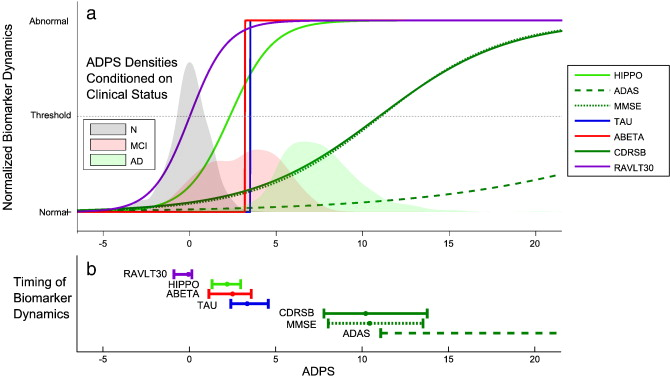
\includegraphics[width=0.8\textwidth,trim=0 80 0 0, clip]{dps_diagram}
   \end{minipage}

   \begin{minipage}[t][\mnpHeight][t]{0.49\linewidth}
    \centering
    \textbf{Manifold-based model}\\ \footnotesize{(Schiratti et al., IPMI, 2015)}
    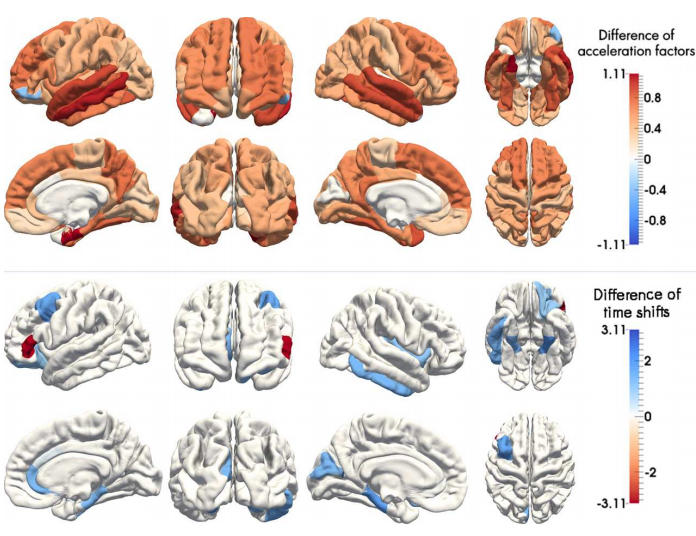
\includegraphics[width=1\textwidth,trim=0 270 0 0, clip]{schiratti}
    
    \vspace{2em}
    
    
   \end{minipage}
   \begin{minipage}[t][\mnpHeight][t]{0.49\linewidth}
    \centering
    \textbf{Self-Modelling Regression}\\ \footnotesize{(Donohue et al., Alz. \& Dementia, 2014)}
    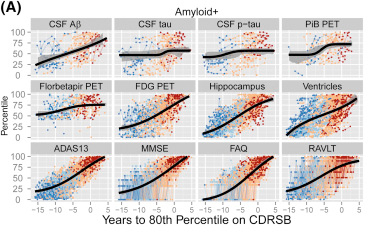
\includegraphics[width=0.8\textwidth]{semor_diagram_cropped}
   \end{minipage}


  \end{figure}
  \end{small}
  
  \vspace{-5em}
  
\end{itemize}

\end{frame}



\begin{frame}
\frametitle{Background - Disease Progression Modelling}

\newcommand{\mnpHeight}{3cm}

\vspace{-3em}
% \textbf{Background}:
\textbf{Voxelwise disease progression model} (Bilgel et al., IPMI, 2015)
\begin{itemize}
  \item Built on PET data measuring amyloid load at each voxel
  \item Estimates a unique trajectory for each voxel
  \item However, it uses a spatial correlation function

  \vspace{2em}
  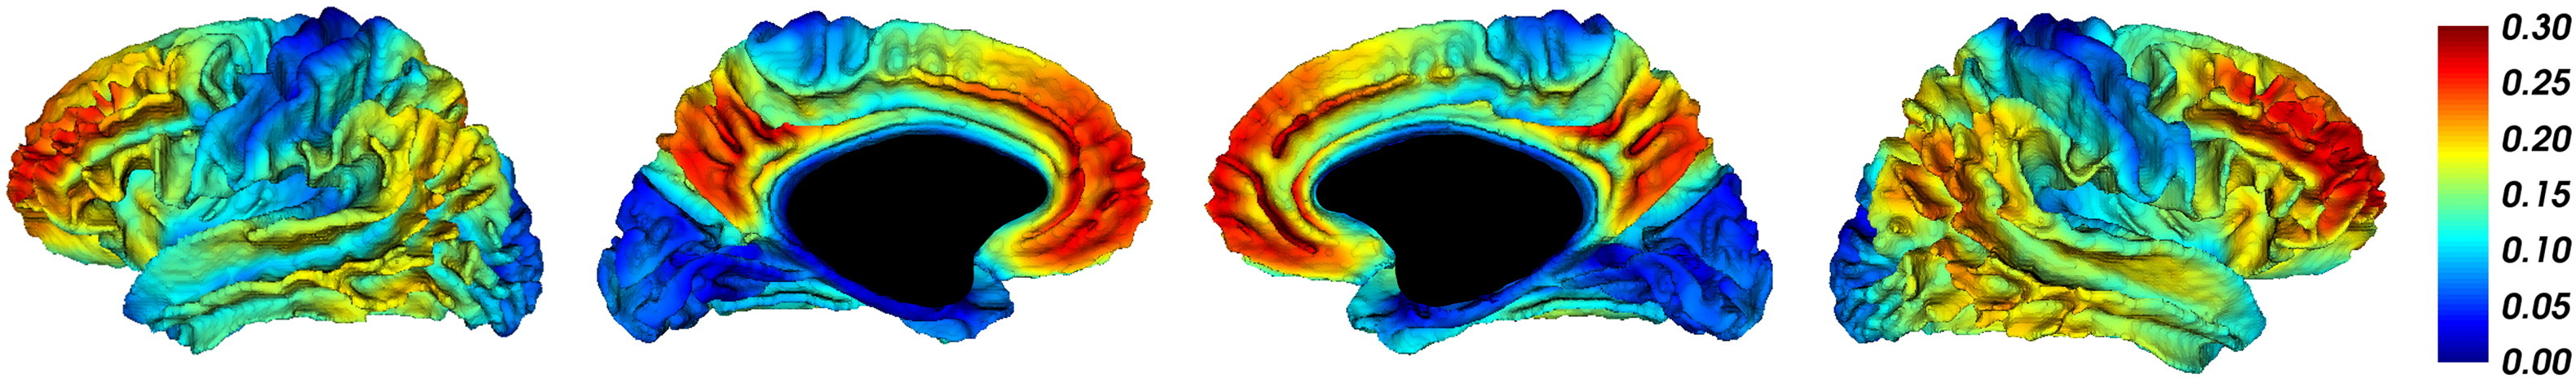
\includegraphics[width=0.85\textwidth]{bilgel_neuroimage}
  \vspace{2em}

  \item We aim to avoid imposing spatial correlation
  
  \end{itemize}



\end{frame}


\newcommand{\outFolder}{../../modelDiagram}
\newcommand{\lw}{0.5mm}

\section{Methods}

\begin{frame}
\frametitle{Methods - Model Description}
% method slide 1

\begin{columns}[T]
%     \hspace{-2em}
    \begin{column}{.7\textwidth}
     %\begin{block}{}
    
    \textbf{Idea}
    \begin{itemize}
      \item Combine two techniques:
      \begin{itemize}
      \item unsupervised learning (clustering)
      \item disease progression modelling
      \end{itemize}
      
      \item Estimate trajectories for each vertex on the cortical surface
      \item Vertex measures cortical thickness at that location

    \end{itemize}
    
    
    \vspace{2em}
   
    \textbf{Method outline}:
    \setbeamertemplate{enumerate items}[default]
     \begin{enumerate}
      \item Each subject has a \emph{disease progression score} (DPS):
      $$s_{ij} = \alpha_i t_{ij} + \beta_i$$
      
      where:
      \begin{itemize}
       \item $s_{ij}$ - disease progression score of subject $i$ at timepoint $j$
       \item $t_{ij}$ - age of subject $i$ at timepoint $j$
       \item $\alpha_i $ - progression speed of subject $i$
       \item $\beta_i $ - time shift of subject $i$
      \end{itemize}
            
     \end{enumerate}
     

    %\end{block}
    \end{column}
    \hspace{-2em}
    \begin{column}{.25\textwidth}
    %\begin{block}{}
    
    \vspace{10em}
    \begin{figure}
    \centering
    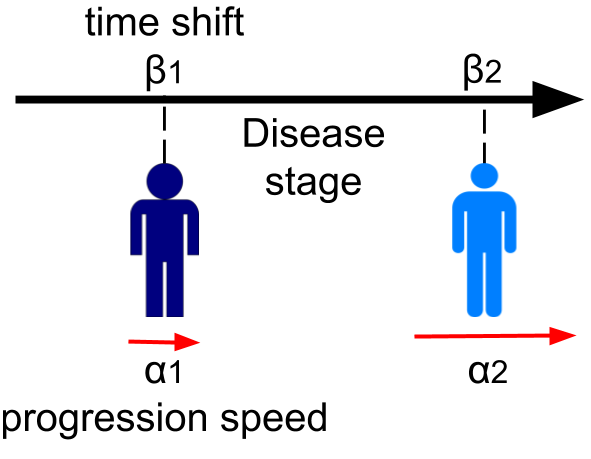
\includegraphics[scale=0.15]{disease_axis.png}
    \end{figure}
    

    %\end{block}
    \end{column}
  \end{columns}

\end{frame}


%%%%%%%%%%%%%%%%%%%%%%%%%%%%%%%%%%%%%%%%%%%%

\begin{frame}
\frametitle{Methods - Model Description}
% method slide 2
\begin{columns}[T]
%     \hspace{-2em}
    \begin{column}{.7\textwidth}
     %\begin{block}{}
    
   
    \textbf{Method outline - continued}:
    \setbeamertemplate{enumerate items}[default]
     \begin{enumerate}
  
      \item[2.] Each cortical thickness measurement $V_l^{ij}$ follows a sigmoidal curve $f(\cdot\ ;\theta)$ along the disease progression:
      
      $$ V_l^{ij} \approx f(s_{ij};\theta_k) = \frac{a_k}{1+exp(-b_k(s-c_k))} + d_k $$
      
      where
      \begin{itemize}
      \item  $V_l^{ij}$ - cortical thickness at location $l$ for subject $i$, timepoint $j$
       \item $\theta_k = [a_k, b_k, c_k, d_k]$ - parameters of $k$-th sigmoid curve
      \end{itemize}
      
      \vspace{2em}
      
      \item[3.] We assume Gaussian noise along the $k$-th trajectory:

      $$p(V_l^{ij} | \alpha_i, \beta_i, \theta_k, \sigma_k) \sim N(f(\alpha_i t_{ij} + \beta_i ; \theta_k), \sigma_k)$$
            
      where:
      \begin{itemize}
       \item $N$ - pdf of the Gaussian distribution
       \item $\sigma_k$ - noise level
       
      \end{itemize}
            
     \end{enumerate}
     

    %\end{block}
    \end{column}
    \hspace{-2em}
    \begin{column}{.25\textwidth}
    %\begin{block}{}
    
    \begin{figure}
    \centering
    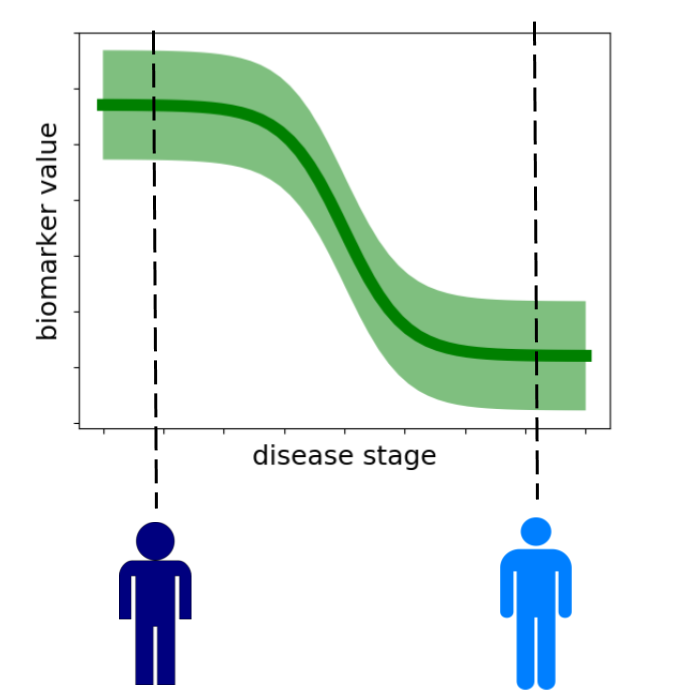
\includegraphics[scale=0.14, trim=120 0 120 0]{Disease_progression_one_sigmoid_confidence.png}
    \end{figure}

    %\end{block}
    \end{column}
  \end{columns}

\end{frame}


%%%%%%%%%%%%%%%%%%%%%%%%%%%%%%%%%%%%%%%%%%%%


\begin{frame}
\frametitle{Methods - Model Description}
% method slide 3

\begin{columns}[T]
%     \hspace{-4em}
    \begin{column}{.75\textwidth} % TODO remove columns here, not needed anymore
     %\begin{block}{}
   
    \setbeamertemplate{enumerate items}[default]
     
    \textbf{Idea:} Group vertices with similar progression dynamics into clusters\\ 
   \vspace{2em}
    \textbf{Method outline - continued}:
   \begin{enumerate}      
      
      \item[4.] Define $Z_l$ as the cluster that generated vertex $l$:
      $$ p(V_l^{ij} | \alpha_i, \beta_i, \theta_{Z_l}, \sigma_{Z_l}, Z_l) \sim N(f(\alpha_i t_{ij} + \beta_i ; \theta_{Z_l}), \sigma_{Z_l}) $$
        where
	\begin{itemize}
	\item $Z_l$ - discreete latent variable assigning vertex $l$ to a cluster $k \in [1 \dots K]$
	\end{itemize}
      \vspace{1em}
      \item[5.] Extend to all subjects and vertices:
  $$  p(V, Z | \alpha, \beta, \theta, \sigma) = \prod_l^L \prod_{(i,j) \in I} N(V_l^{ij} | f(\alpha_i t_{ij} + \beta_i ; \theta_{Z_l}), \sigma_{Z_l}) $$
  where
  \begin{itemize}
  \item $L$ - the total number of vertices on the cortical surface
  \item $I = {(i,j)}$ - set of available timepoints for each subject $i$ and timepoint $j$   
  \item we assume independence across subjects and voxels in different clusters
  \end{itemize}
     
     \end{enumerate}
     

    %\end{block}
    \end{column}
    \hspace{-3em}
    \begin{column}{.25\textwidth}
    %\begin{block}{}

%         \node  (brain) at (1.3,4.5) {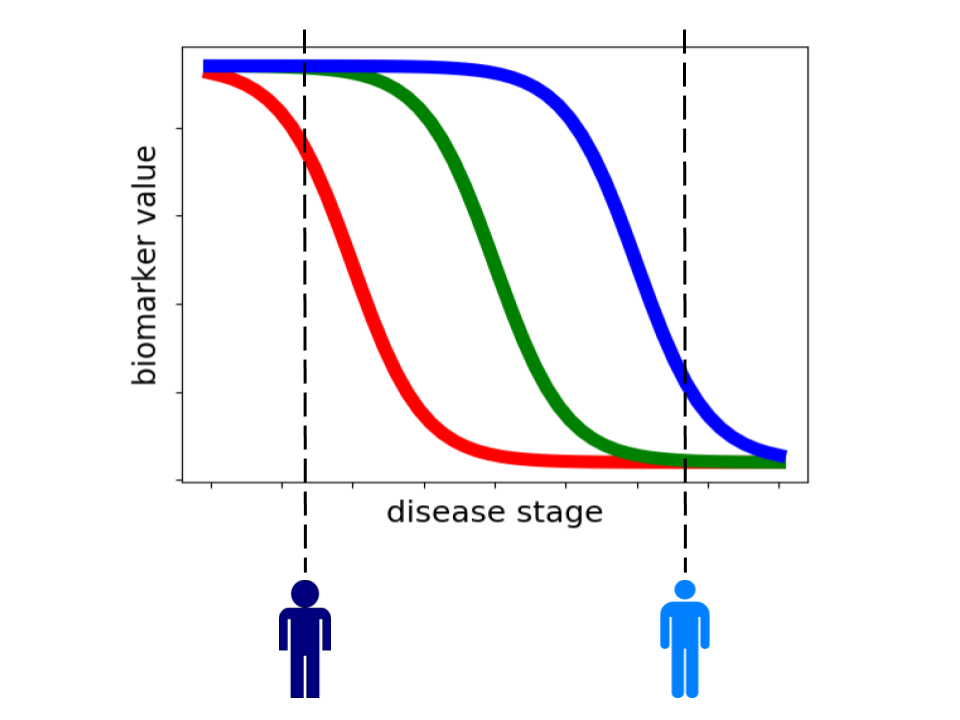
\includegraphics[scale=0.1]{disease_progression_staging.png}};
    
    \begin{figure}
    \centering
    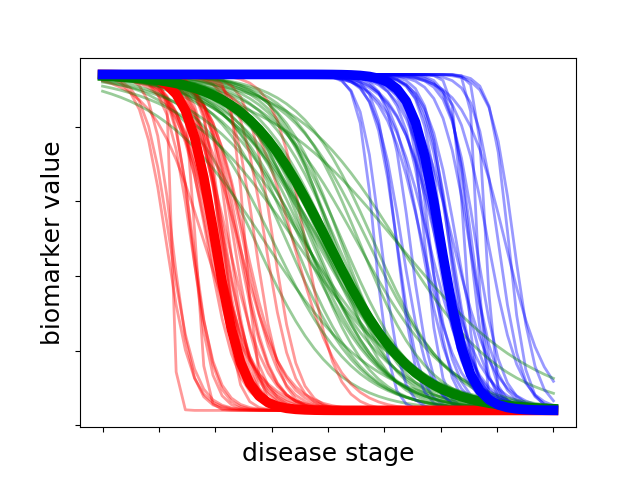
\includegraphics[scale=0.22, trim=120 0 120 70]{\outFolder/sigManyBiomkClustering.png}
    \end{figure}

    %\end{block}
    \end{column}
  \end{columns}
  
%   \begin{itemize}
% 
%   
%   \end{itemize}


\end{frame}

%%%%%%%%%%%%%%%%%%%%%%%%%%%%%%%%%%%%%%%%%%%%%%


\begin{frame}
\frametitle{Methods - Model Description}
% method slide 4

\begin{columns}[T]
    \hspace{-4em}
    \begin{column}{.65\textwidth}
     %\begin{block}{}
   
    \textbf{Method outline - continued}:
    \setbeamertemplate{enumerate items}[default]
     \begin{enumerate}      
          
      \item[6.] Marginalise over the hidden variables $Z_l$ (cluster assignments):
      \small{$$p(V|\alpha, \beta, \theta, \sigma) = \prod_{l=1}^L \sum_{k=1}^K p(Z_l = k) \prod_{(i,j) \in I} N(V_l^{ij} | f(\alpha_i t_{ij} + \beta_i \ ; \theta_k), \sigma_k)$$}
       \end{enumerate}
       
    \textbf{Summary}:
      \begin{enumerate}  
       \item Model clusters vertices on the brain surface according to disease progression dynamics
       \begin{itemize}
        \item No assumptions on spatial correlation
       \end{itemize}
       \item Model estimates one trajectory for each cluster
       \item Model estimates subject progression scores
       \item Parameters to estimate: $\left[\alpha, \beta, \theta, \sigma \right]$
      
     \end{enumerate}
     

    %\end{block}
    \end{column}
    \hspace{-3em}
    \begin{column}{.25\textwidth}
    
    %     \vspace{-3em}
    \begin{figure}
%     \centering
%     \hspace{-4.5em}
    \begin{tikzpicture}[scale=0.8]
     \draw[line width=\lw] (-0.1,0) arc (-20:20:2) node (A1) {};
     \draw[line width=\lw] (1.7,0) arc (-20:20:2)  node (A2) {} ;
     \draw[,fill=red] (0.22,0.10) circle (0.15cm);
     \draw[,fill=red] (0.32,0.50) circle (0.15cm);
     \draw[,fill=blue] (0.32,0.90) circle (0.15cm);
     \draw[,fill=red] (0.22,1.30) circle (0.15cm);
     \draw[,fill=red] (0.62,0.10) circle (0.15cm);
     \draw[,fill=blue] (0.72,0.50) circle (0.15cm);
     \draw[,fill=blue] (0.72,0.90) circle (0.15cm);
     \draw[,fill=red] (0.62,1.30) circle (0.15cm);
     \draw[,fill=green] (1.02,0.10) circle (0.15cm);
     \draw[,fill=red] (1.12,0.50) circle (0.15cm);
     \draw[,fill=red] (1.12,0.90) circle (0.15cm);
     \draw[,fill=green] (1.02,1.30) circle (0.15cm);
     \draw[,fill=green] (1.42,0.10) circle (0.15cm);
     \draw[,fill=green] (1.52,0.50) circle (0.15cm);
     \draw[,fill=green] (1.52,0.90) circle (0.15cm);
     \draw[,fill=blue] (1.42,1.30) circle (0.15cm);
     \node (sig0) at (1.20,2.70) {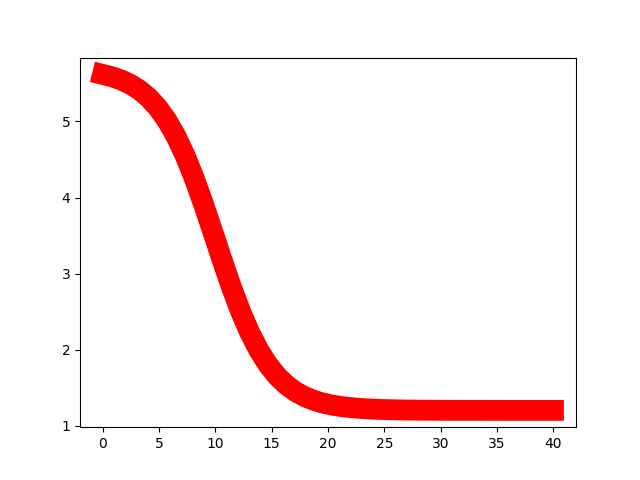
\includegraphics[scale=0.08, trim=70 70 70 0]{\outFolder/sig0.png}};
    \node  (traj) at (sig0.north) {\scriptsize{Traj. 0}}; 
     \node (sig1) at (2.75,2.25) {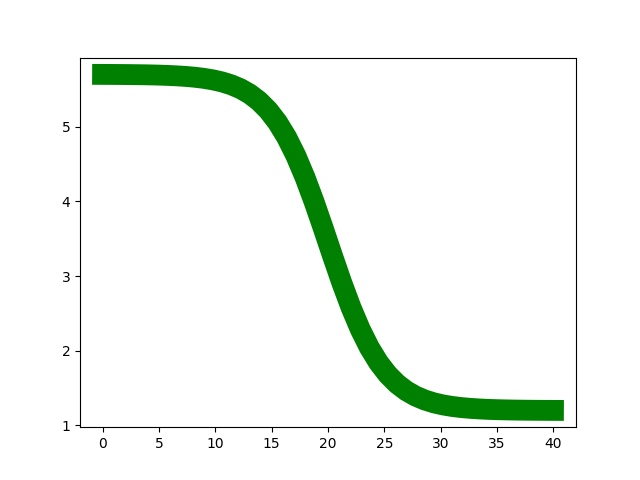
\includegraphics[scale=0.08, trim=70 70 70 0]{\outFolder/sig1.png}};
    \node  (traj) at (sig1.north) {\scriptsize{Traj. 1}}; 
     \node (sig2) at (3.00,0.80) {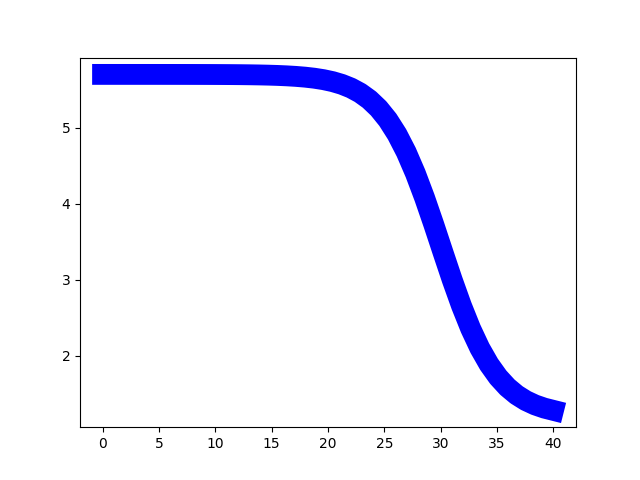
\includegraphics[scale=0.08, trim=70 70 70 0]{\outFolder/sig2.png}};
    \node  (traj) at (sig2.north) {\scriptsize{Traj. 2}}; 


    \draw[dotted, line width=0.6, color=red] (sig0.south west) -- (-0.1,1.5);
    \draw[dotted, line width=0.6, color=red] (sig0.south east) -- (1.8,1.5);

    \draw[dotted, line width=0.6, color=green] (sig1.west) -- (01,1.5);
    \draw[dotted, line width=0.6, color=green] (sig1.south) -- (1.8,0);

    \draw[dotted, line width=0.6, color=blue] (sig2.north west) -- (1.6,1.5);
    \draw[dotted, line width=0.6, color=blue] (sig2.south west) -- (0.7,0.3);

    \node  (vertices_label) at (0.8,1.8) {\scriptsize{Vertices}};


    % draw the bran and the magnification from it
    \node  (brain) at (0.8,-1.1) {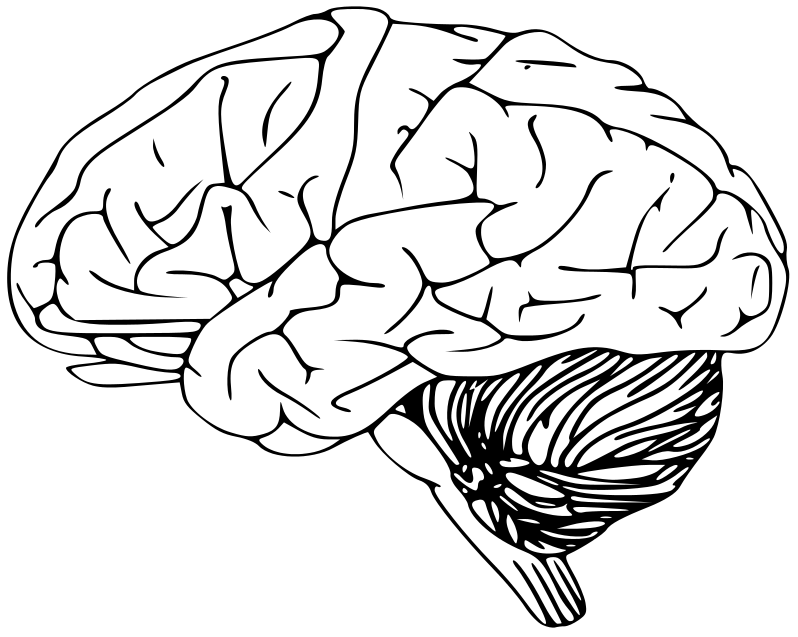
\includegraphics[scale=0.06]{\outFolder/brain.png}};

    \draw (0.8,-0.8) circle (0.15cm) node (C) {};
    \draw[dotted, line width=0.8, color=black] (C.west) -- (-0.1,-0.15);
    \draw[dotted, line width=0.8, color=black] (C.east) -- (1.6,-0.15);
    
   \end{tikzpicture}
  \end{figure}
  \vspace{-2em}

    %\end{block}
    \end{column}
  \end{columns}

\end{frame}

%%%%%%%%%%%%%%%%%%%%%%%%%%%%%%%%%%%%%%%%%%%%%%

\newcommand*{\scaleBrainImg}{0.2}
\newcommand*{\scaleAllSubfigsImg}{1}
% scale parameter for the circles and the gradient
\tikzset{every picture/.append style={scale=0.4}}



\begin{frame}
\frametitle{Methods - Fitting Procedure}

% \newcommand{\mycirc}[2]{\draw (#1,#2) circle (3cm);}

% \newcommand{\outFolder}{.}
     
    \vspace{1em} 
    \textbf{Model fitting with Expectation-Maximisation (EM)}:
    \vspace{1em}
    \begin{itemize}
    \item \textbf{E-step}:
    \begin{itemize}
     \item Estimate vertex assignment to clusters:
     
     \begin{equation}
 z_{lk} =  p(Z_l = k|V_l,\Theta^{old}) =  \frac{\prod_{(i,j) \in I} N(V_l^{ij} | f(\alpha_i^{old} t_{ij} + \beta_i^{old} | \theta_k^{old}), \sigma_k^{old})}{\sum_{m=1}^K \prod_{i,j \in I} N(V_l^{ij} | f(\alpha_i^{old} t_{ij} + \beta_i^{old} | \theta_m^{old}), \sigma_m^{old})}
\end{equation}

    \end{itemize}
    \item \textbf{M-step}:
    \begin{itemize}
     \item Update trajectories:
     
     \begin{equation}
 \label{eq:theta}
 \theta_k = \argmin_{\theta_k} \left[\sum_{l=1}^L z_{lk} \sum_{(i,j) \in I} (V_l^{ij} - f(\alpha_i t_{ij} + \beta_i | \theta_k))^2 \right] - log\ p(\theta_k) 
\end{equation}
     
     \item Update subject progression scores:
     
     \begin{equation}
\label{eq:alpha}
 \alpha_i, \beta_i = \argmin_{\alpha_i, \beta_i}  \left[ \sum_{l=1}^L \sum_{k=1}^K z_{lk} \frac{1}{2\sigma_k^2} \sum_{j \in I_i} (V_l^{ij} - f(\alpha_i t_{ij} + \beta_i | \theta_k))^2\right] - log\ p(\alpha_i, \beta_i)
\end{equation}
     
    \end{itemize}
    \end{itemize}
    %\end{block}


\end{frame}


\begin{frame}
\frametitle{Methods - Numerical Optimisation and Initialisation}

\textbf{M-step - Numerical optimisation} 
\begin{itemize}
\item M-step has no analytical solution
\item Perform numerical optimisation with Broyden-Fletcher-Goldfarb-Shanno (BFGS):
\begin{itemize}
  \item fast convergence
  \item uses first derivative of objective function
\end{itemize}
\item EM still converges with partial M-step
\end{itemize}
%\end{block}

\vfill

\textbf{Initialisation}

\begin{itemize}
 \item We set $\alpha_i=1$ and $\beta_i=0$, $\forall i$
 \item We initialise $z_{lk} = p(Z_l = k|V_l,\Theta^{old})$ using k-means clustering
 \begin{itemize}
  \item feature vector for vertex $l$: $\left[ V_l^{ij} | (i,j) \in I \right]$ (measurements for all subjects at that location)
 \end{itemize}

 \item Estimate the optimal number of clusters with the Bayesian Information Criterion (BIC)
 \begin{itemize}
  \item Number of parameters: $5K + 2S$
 \end{itemize}

\end{itemize}

\end{frame}


\begin{frame}
\frametitle{Outline - Results}

\begin{enumerate}
  \item Simulation tests using synthetic data
  \vfill
  \item Results on two datasets:
  \begin{itemize}
   \item Alzheimer's Disease Neuroimaging Initiative (ADNI)
   \item Dementia Research Center, University College London (UCL DRC)
  \end{itemize}
  \vfill
  \item Model validation
  \begin{itemize}
   \item Robustness
   \item Staging consistency
%    \item Model comparison
  \end{itemize}

  \vfill
  \item Recent results (not included in paper)
\end{enumerate}

\end{frame}

    
\section{Results}
\begin{frame}
\frametitle{Preliminary Simulation}

\begin{itemize}
 \item Simulated data from 1,000 vertices generated from 3 clusters:
 \begin{enumerate}
  \item sampled age and shift parameters from 300 subjects with 4 timepoints (each timepoint 1 year apart), with $t_{i1} \sim U(40,80)$, $\alpha_i \sim N(1, 0.05)$, $\beta_i \sim N(0, 10)$ 
  \item generated three sigmoidal trajectories with different center points and slopes (red lines) 
  \item generated a random cluster assignment for $L = 1,000$ vertices 
  \item sampled $L$ perturbed trajectories $\theta_l$ from the original trajectories, one for each vertex (gray lines) 
  \item sampled subject data for every vertex $l$ from its corresponding perturbed trajectory $\theta_l$ with $\sigma_l = 0.5$
 \end{enumerate}
 \item Model was able to recover the:
 \begin{itemize}
  \item underlying trajectories, Fig. (a)
  \item subject progression scores, Fig. (b)
 \end{itemize}

 
\end{itemize}

\begin{figure}
\begin{subfigure}[b]{0.75\textwidth}
  \hspace{-1em}
  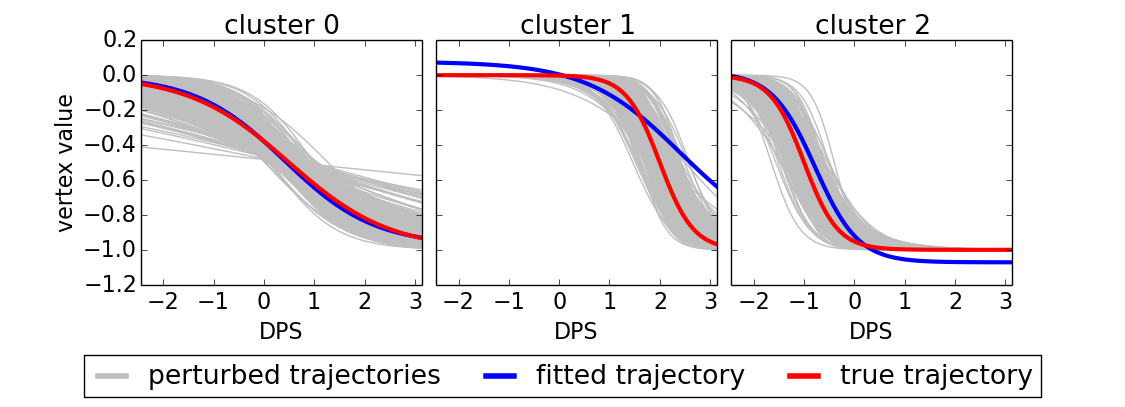
\includegraphics[width=1\textwidth]{figures/synThetaRes_gensigInitk-meansCl3Pr1Ra0_VWDPMStd.png}
  \caption{}
  \label{fig:synThetaRes}
\end{subfigure}
\hspace{-2em}
\begin{subfigure}[b]{0.24\textwidth}
\centering
  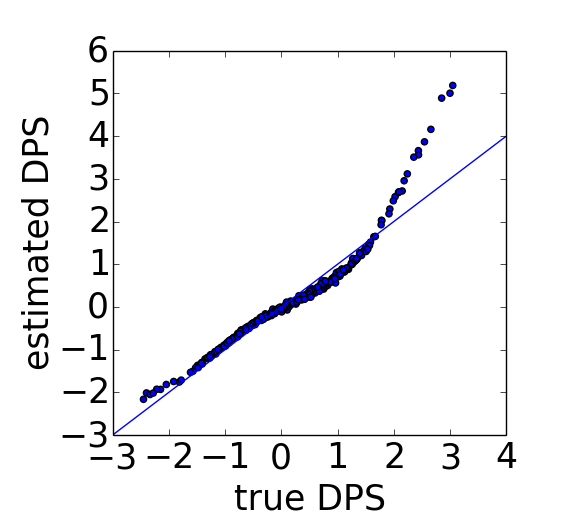
\includegraphics[width=1.1\textwidth]{figures/synShiftsRes_gensigInitk-meansCl3Pr1Ra0_VWDPMStd.png}
  \vspace{0.9em}
  \caption{}
  \label{fig:synShiftRes}
\end{subfigure}
\end{figure}
\end{frame}

%%%%%%%%%%%%%%%%%%%%%%%%%%%%%%


\begin{frame}
\frametitle{Simulations - Stress Tests}


 \textbf{Hypothesis}: Model will perform worse when:
 \begin{itemize}
  \item the trajectories are very similar to each other
  \item number of clusters is large
  \item number of subjects is decreasing
 \end{itemize}

%  \vfill
 
 \textbf{Method}: Performed several "stress tests" for each scenario:

%  \vfill
 \begin{figure}
\centering
\begin{subfigure}{0.3\textwidth}
\centering
\small{Trajectories becoming similar}\\
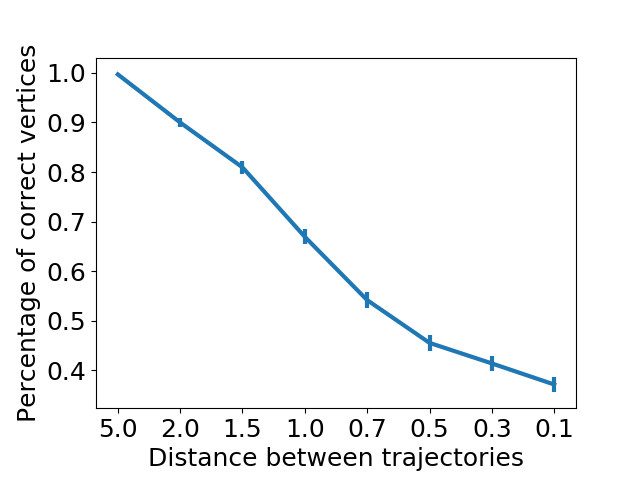
\includegraphics[scale=0.22]{figures/synth/correctVertices_trajCent}
\caption{}
\end{subfigure}
\begin{subfigure}{0.3\textwidth}
\centering
\small{Increasing number of clusters}
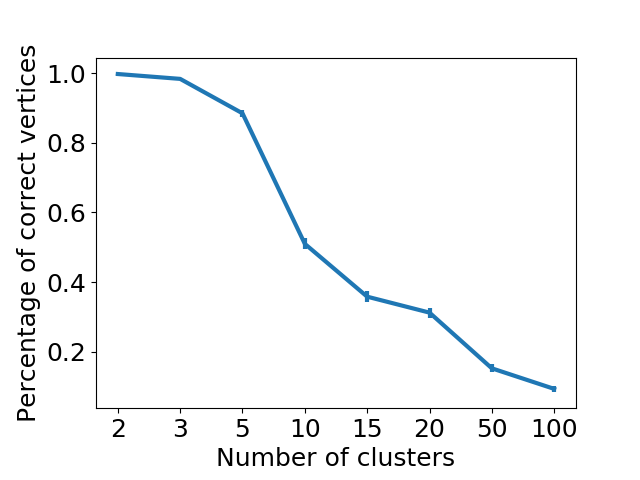
\includegraphics[scale=0.22]{figures/synth/correctVertices_nrClust}
\caption{}
\end{subfigure}
\begin{subfigure}{0.3\textwidth}
\centering
\small{Decreasing number of subjects}
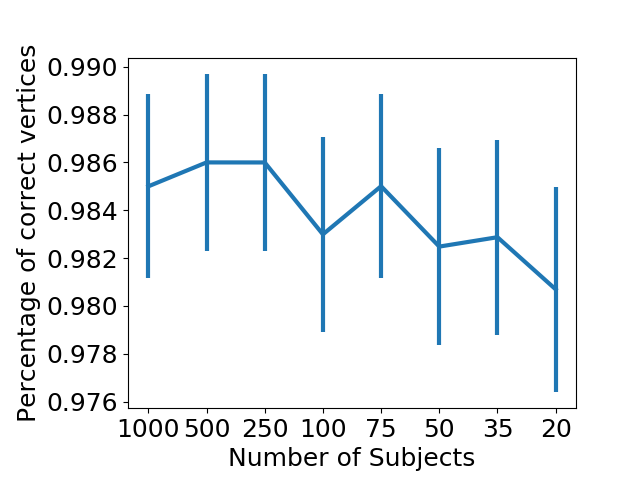
\includegraphics[scale=0.22]{figures/synth/correctVertices_nrSubj}
\caption{}
\end{subfigure}

% \vfill

\end{figure}

  \textbf{Conclusion}: 
  \begin{itemize}
  \item Model performance decreases when:
    \begin{itemize}
      \item the trajectories become more similar
      \item number of clusters increases
    \end{itemize}
  \item However, performance is not affected by the number of subjects
  \end{itemize}
  
\end{frame}


%%%%%%%%%%%%%%%%%%%%%%%%%%%%%%%%%%%%%%%%%%%%%%%%%%%%%%%%%%%

\begin{frame}
\frametitle{Application to ADNI and UCL DRC datasets}

\vspace{1em}
\textbf{Alzheimer's Disease Neuroimaging Initiative (ADNI) dataset}:

\begin{table}
\centering
\begin{tabular}{ c |c | c | c} 
& Number of Subjects & Number of Scans & Age at baseline (years)\\
\hline
Controls & 138 & 4.3 & 76.3\\ 
MCI & 235 & 4.6 & 74.8\\ 
AD & 81 & 3.5 & 75.8\\ 
\end{tabular}
\label{tab:adni_demographics}
\end{table}

\vspace{1em}

\textbf{Dementia Research Center, University College London (UCL DRC) dataset}:
% \begin{itemize}
%  \item T1 scans from 31 healthy controls, 32 PCA and 24 tAD subjects.
%  \item Average of 5.26 scans per subject
% \end{itemize}

\begin{table}
\centering
\begin{tabular}{ c |c | c | c } 
& Number of Subjects & Number of Scans & Age at baseline (years)\\
\hline
Controls & 31 & 5.0 & 66.3\\ 
PCA & 32 & 4.1 & 62.6\\ 
AD & 24 & 5.4 & 71.2\\ 
\end{tabular}
\label{tab:drc_demographics}
\end{table}

\vspace{1em}

\textbf{Preprocessing}:
\begin{itemize}
 \item Logitudinally registered all MRI images to a common template using Freesurfer
 \item Extracted vertexwise cortical thickness measurements
 \item Cortical thickness values at each vertex were standardised with respect to controls
\end{itemize}

\end{frame}

%%%%%%%%%%%%%%%%%%%%%%%%%%%%%%%%%%%%%%%%%%%%%%%%%%%%%%%%%%%

\begin{frame}
\frametitle{Results - ADNI and UCL DRC Cohorts}


\newcommand{\scalingFactor}{0.9}

\newcommand{\gradLimLeft}{-1.6}
\newcommand{\gradLimRight}{1.6}

% \newcommand{\scalingFactorLeftFig}{1.2}
\newcommand{\scalingFactorBrains}{1.0}
\newcommand{\scalingFactorTraj}{1}

\vspace{-0.5em}

% \vspace{-1em}
% FWHM0 avg thickness map MCI & AD
\begin{figure}[h]
  \centering

  % do the legend colorbar
  \begin{subfigure}[b]{\textwidth}
   \centering
  \begin{tikzpicture}[scale=1.9*\scalingFactor, every node/.style={scale=0.8*\scalingFactor}]
    \shade[left color=red,right color=green] (\gradLimLeft,2.5) rectangle (0,2.75);
    \shade[left color=green,right color=blue] (0,2.5) rectangle (\gradLimRight,2.75);
    \node[inner sep=0] (corr_text) at (\gradLimLeft,2.25) {cluster 0};
    \node[inner sep=0] (corr_text) at (0,2.25) {cluster 1};
    \node[inner sep=0] (corr_text) at (\gradLimRight,2.25) {cluster 2};
    \node[inner sep=0] (corr_text) at (\gradLimLeft,3) {rapid atrophy};
    \node[inner sep=0] (corr_text) at (\gradLimRight,3) {slow atrophy};
  \end{tikzpicture}
%     \caption{}
%       \label{fig:adniClust}
  \vspace{1em}
  \end{subfigure}
  
  %%%%%%%%%%%%%%%%%%% BRAINS %%%%%%%%%%%%%%5%%%%%%
  
  %%%%%%%% slide 1 %%%%%%%%%%%%%
  
  \begin{subfigure}[b]{0.3\textwidth}
   \centering
  \begin{tikzpicture}[scale=\scalingFactor, every node/.style={scale=\scalingFactor}]
    \node[inner sep=0] (image) at (0,0) {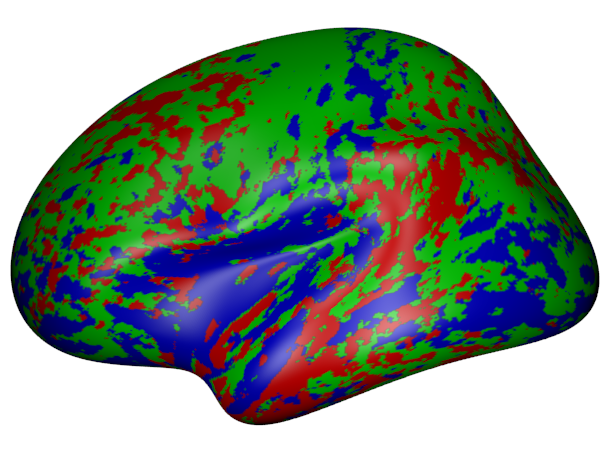
\includegraphics[width=\scalingFactorBrains\textwidth]{figures/blend14_adniThavgFWHM0InithistCl3Pr0Ra1_VWDPMStd.png}}; 
    \node[inner sep=0] (label) at (0,3.5) {tAD - ADNI};
  \end{tikzpicture}
%     \caption{}
%       \label{fig:adniClust}
  \end{subfigure}
   \begin{subfigure}[b]{0.3\textwidth}
  \centering
  \begin{tikzpicture}[scale=\scalingFactor, every node/.style={scale=\scalingFactor}]
    \node[inner sep=0] (corr_text) at (0,0) {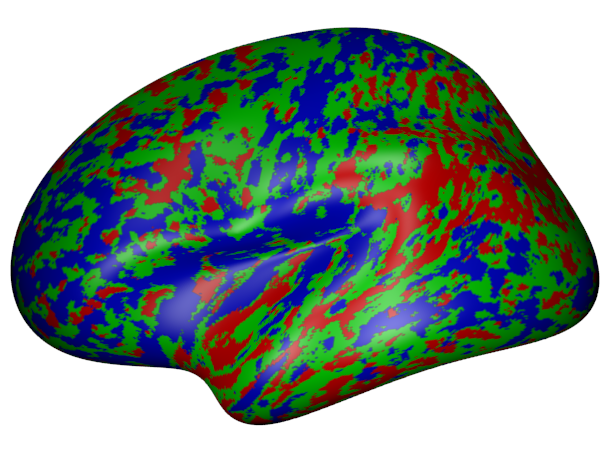
\includegraphics[width=\scalingFactorBrains\textwidth]{figures/drcThavgFWHM0InithistCl3Pr0Ra1_VWDPMStdAD_blend24.png}};
    \node[inner sep=0] (label) at (0,3.5) {tAD - UCL DRC dataset};
  \end{tikzpicture}
%     \caption{}
%       \label{fig:drcClustAD}
  \end{subfigure}
   \begin{subfigure}[b]{0.3\textwidth}
  \centering
  \begin{tikzpicture}[scale=\scalingFactor, every node/.style={scale=\scalingFactor}]
    \node[inner sep=0] (corr_text) at (0,0) {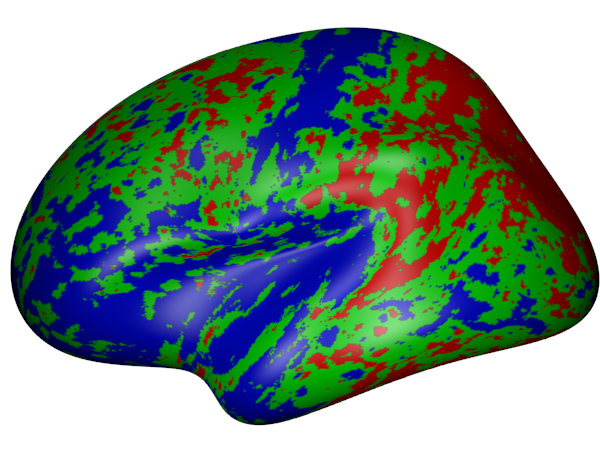
\includegraphics[width=\scalingFactorBrains\textwidth]{figures/drcThavgFWHM0InithistCl3Pr0Ra1_VWDPMStdPCA_blend24.png}};
    \node[inner sep=0] (label) at (0,3.5) {PCA - UCL DRC dataset};
  \end{tikzpicture}
%     \caption{}
%       \label{fig:drcClustPCA}
  \end{subfigure}
  
  %%%%%%%%%%%%%%%%%%%%%% trajectories %%%%%%%%%%%%%%%%%%%%%%%
  
    \begin{subfigure}[b]{0.3\textwidth}
    \centering
%     \vspace{-2em}
    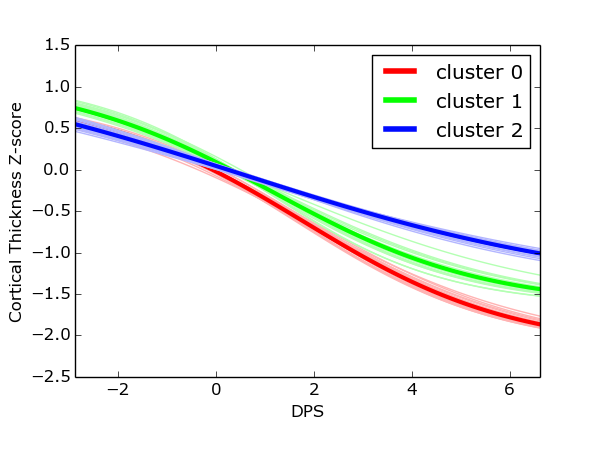
\includegraphics[width=\scalingFactor\textwidth]{figures/trajSamplesOneFig_adniThavgFWHM0InithistCl3Pr0Ra1_VWDPMStd.png}
%     \caption{}
%       \label{fig:adniTraj}
  \end{subfigure}
      \begin{subfigure}[b]{0.3\textwidth}
    \centering
%     \vspace{-2em}
    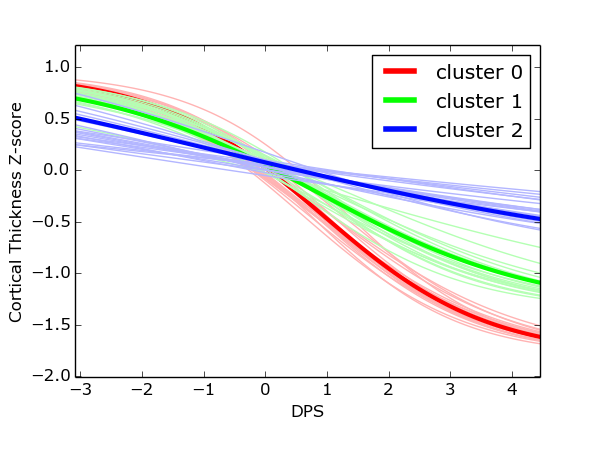
\includegraphics[width=\scalingFactor\textwidth]{figures/trajSamplesOneFig_drcThavgFWHM0InithistCl3Pr0Ra1_VWDPMStdAD.png}
%     \caption{}
%       \label{fig:drcTrajAD}
  \end{subfigure}
    \begin{subfigure}[b]{0.3\textwidth}
    \centering
%     \vspace{-2em}
    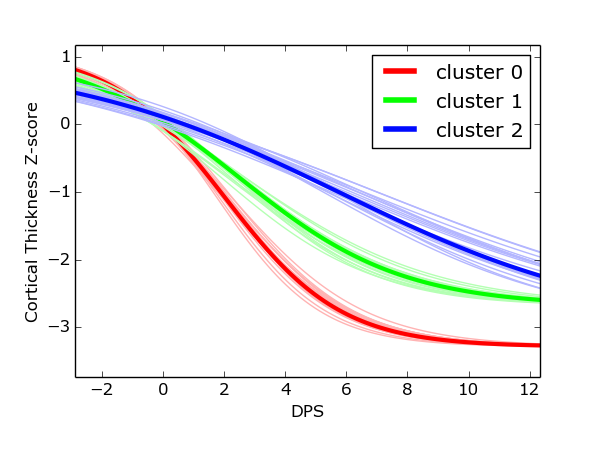
\includegraphics[width=\scalingFactor\textwidth]{figures/trajSamplesOneFig_drcThavgFWHM0InithistCl3Pr0Ra1_VWDPMStdPCA.png}
%     \caption{}
%       \label{fig:drcTrajPCA}
  \end{subfigure}
  
%   \caption{}
%   \label{fig:clustTrajAll}

\end{figure}

\vspace{-1em}

\textbf{Conclusions:}
\begin{itemize}
 \item Similar patterns of atrophy in tAD in two independent datasets: ADNI and UCL DRC
 \item Distinct patterns of atrophy in two different diseases: typical AD and Posterior Cortical Atrophy
\end{itemize}



\end{frame}

%%%%%%%%%%%%%%%%%%%%%%%%%%%%%%%%%%%%%%%%%%%%%%%%%%%%%%%%%%%%%5


\begin{frame}
\frametitle{Results - ADNI and UCL DRC Cohorts}

\newcommand{\scalingFactor}{0.9}

\newcommand{\gradLimLeft}{-1.6}
\newcommand{\gradLimRight}{1.6}

% \newcommand{\scalingFactorLeftFig}{1.2}
\newcommand{\scalingFactorBrains}{1.0}
\newcommand{\scalingFactorTraj}{1}

\vspace{-0.5em}

% \vspace{-1em}
% FWHM0 avg thickness map MCI & AD
\begin{figure}[h]
  \centering

  % do the legend colorbar
  \begin{subfigure}[b]{\textwidth}
   \centering
  \begin{tikzpicture}[scale=1.9*\scalingFactor, every node/.style={scale=0.8*\scalingFactor}]
    \shade[left color=red,right color=green] (\gradLimLeft,2.5) rectangle (0,2.75);
    \shade[left color=green,right color=blue] (0,2.5) rectangle (\gradLimRight,2.75);
    \node[inner sep=0] (corr_text) at (\gradLimLeft,2.25) {cluster 0};
    \node[inner sep=0] (corr_text) at (0,2.25) {cluster 1};
    \node[inner sep=0] (corr_text) at (\gradLimRight,2.25) {cluster 2};
    \node[inner sep=0] (corr_text) at (\gradLimLeft,3) {rapid atrophy};
    \node[inner sep=0] (corr_text) at (\gradLimRight,3) {slow atrophy};
  \end{tikzpicture}
%     \caption{}
%       \label{fig:adniClust}
  \vspace{1em}
  \end{subfigure}
  
  %%%%%%%%%%%%%%%%%%% BRAINS %%%%%%%%%%%%%%5%%%%%%
  
  %%%%%%%% slide 2 %%%%%%%%%%%%%
  
  \begin{subfigure}[b]{0.3\textwidth}
   \centering
  \begin{tikzpicture}[scale=\scalingFactor, every node/.style={scale=\scalingFactor}]
    \node[inner sep=0] (image) at (0,0) {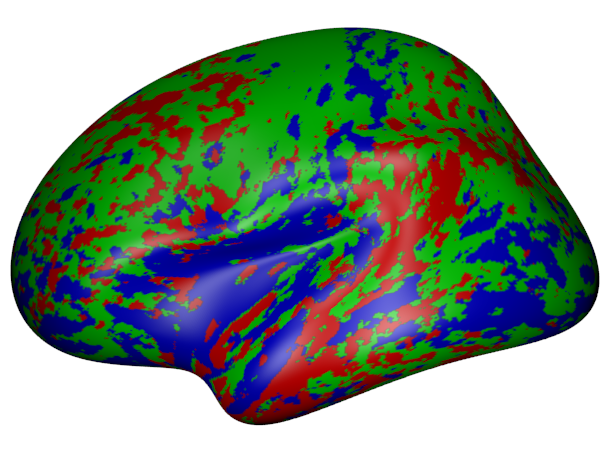
\includegraphics[width=\scalingFactorBrains\textwidth]{figures/blend14_adniThavgFWHM0InithistCl3Pr0Ra1_VWDPMStd.png}}; 
    \node[inner sep=0] (label) at (0,3.5) {tAD - ADNI};
    \draw[line width=0.4mm] (0,-0.5) rectangle (4,2.5);
  \end{tikzpicture}
%     \caption{}
%       \label{fig:adniClust}
  \end{subfigure}
   \begin{subfigure}[b]{0.3\textwidth}
  \centering
  \begin{tikzpicture}[scale=\scalingFactor, every node/.style={scale=\scalingFactor}]
    \node[inner sep=0] (corr_text) at (0,0) {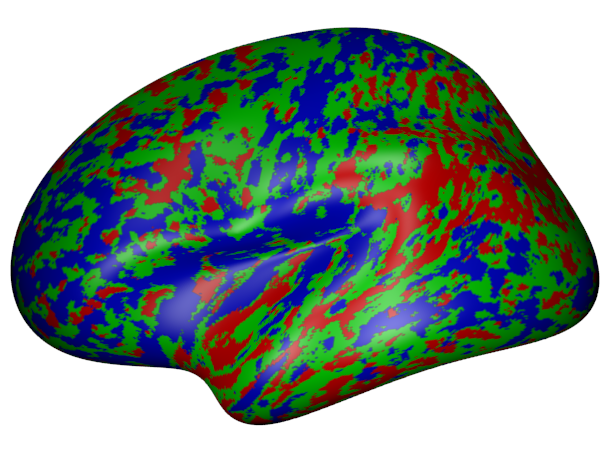
\includegraphics[width=\scalingFactorBrains\textwidth]{figures/drcThavgFWHM0InithistCl3Pr0Ra1_VWDPMStdAD_blend24.png}};
    \node[inner sep=0] (label) at (0,3.5) {tAD - UCL DRC dataset};
    \draw[line width=0.4mm] (0,-0.5) rectangle (4,2.5);
  \end{tikzpicture}
%     \caption{}
%       \label{fig:drcClustAD}
  \end{subfigure}
   \begin{subfigure}[b]{0.3\textwidth}
  \centering
  \begin{tikzpicture}[scale=\scalingFactor, every node/.style={scale=\scalingFactor}]
    \node[inner sep=0] (corr_text) at (0,0) {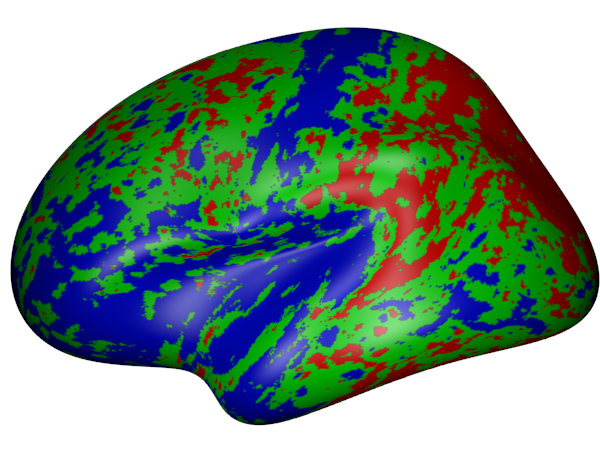
\includegraphics[width=\scalingFactorBrains\textwidth]{figures/drcThavgFWHM0InithistCl3Pr0Ra1_VWDPMStdPCA_blend24.png}};
    \node[inner sep=0] (label) at (0,3.5) {PCA - UCL DRC dataset};
    \draw[line width=0.4mm] (0,-0.5) rectangle (4,2.5);
  \end{tikzpicture}
%     \caption{}
%       \label{fig:drcClustPCA}
  \end{subfigure}
  
  %%%%%%%%%%%%%%%%%%%%%% trajectories %%%%%%%%%%%%%%%%%%%%%%%
  
    \begin{subfigure}[b]{0.3\textwidth}
    \centering
%     \vspace{-2em}
    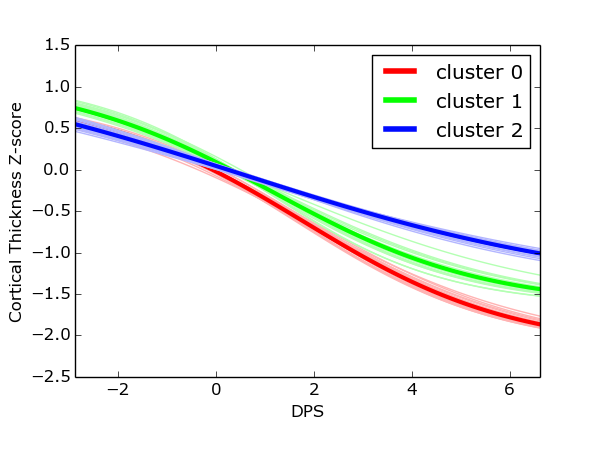
\includegraphics[width=\scalingFactor\textwidth]{figures/trajSamplesOneFig_adniThavgFWHM0InithistCl3Pr0Ra1_VWDPMStd.png}
%     \caption{}
%       \label{fig:adniTraj}
  \end{subfigure}
      \begin{subfigure}[b]{0.3\textwidth}
    \centering
%     \vspace{-2em}
    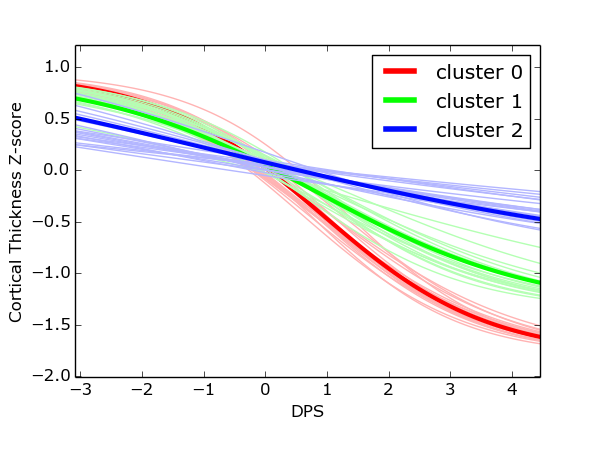
\includegraphics[width=\scalingFactor\textwidth]{figures/trajSamplesOneFig_drcThavgFWHM0InithistCl3Pr0Ra1_VWDPMStdAD.png}
%     \caption{}
%       \label{fig:drcTrajAD}
  \end{subfigure}
    \begin{subfigure}[b]{0.3\textwidth}
    \centering
%     \vspace{-2em}
    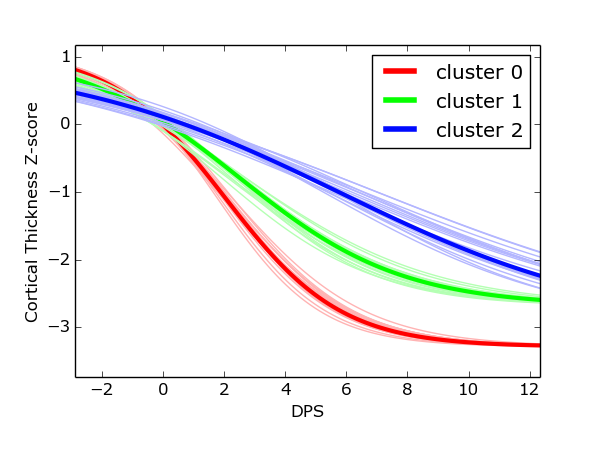
\includegraphics[width=\scalingFactor\textwidth]{figures/trajSamplesOneFig_drcThavgFWHM0InithistCl3Pr0Ra1_VWDPMStdPCA.png}
%     \caption{}
%       \label{fig:drcTrajPCA}
  \end{subfigure}
  
%   \caption{}
%   \label{fig:clustTrajAll}

\end{figure}

\vspace{-1em}

\textbf{Conclusions:}
\begin{itemize}
 \item Similar patterns of atrophy in tAD in two independent datasets: ADNI and UCL DRC
 \item Distinct patterns of atrophy in two different diseases: typical AD and Posterior Cortical Atrophy
\end{itemize}


\end{frame}

%%%%%%%%%%%%%%%%%%%%%%%%%%%%%%%%%%%%%%%%%%%%%%%%%%%%%%%%%%%%%5

\begin{frame}
\frametitle{Results - ADNI and UCL DRC Cohorts}

\newcommand{\scalingFactor}{0.9}

\newcommand{\gradLimLeft}{-1.6}
\newcommand{\gradLimRight}{1.6}

% \newcommand{\scalingFactorLeftFig}{1.2}
\newcommand{\scalingFactorBrains}{1}
\newcommand{\scalingFactorTraj}{1}

\vspace{-0.5em}
% FWHM0 avg thickness map MCI & AD
\begin{figure}[h]
  \centering

  % do the legend colorbar
  \begin{subfigure}[b]{\textwidth}
   \centering
  \begin{tikzpicture}[scale=1.9*\scalingFactor, every node/.style={scale=0.8*\scalingFactor}]
    \shade[left color=red,right color=green] (\gradLimLeft,2.5) rectangle (0,2.75);
    \shade[left color=green,right color=blue] (0,2.5) rectangle (\gradLimRight,2.75);
    \node[inner sep=0] (corr_text) at (\gradLimLeft,2.25) {cluster 0};
    \node[inner sep=0] (corr_text) at (0,2.25) {cluster 1};
    \node[inner sep=0] (corr_text) at (\gradLimRight,2.25) {cluster 2};
    \node[inner sep=0] (corr_text) at (\gradLimLeft,3) {rapid atrophy};
    \node[inner sep=0] (corr_text) at (\gradLimRight,3) {slow atrophy};
  \end{tikzpicture}
%     \caption{}
%       \label{fig:adniClust}
  \vspace{1em}
  \end{subfigure}
  
  %%%%%%%%%%%%%%%%%%% BRAINS %%%%%%%%%%%%%%5%%%%%%
  
  %%%%%%%% slide 3 %%%%%%%%%%%%%
  
  \begin{subfigure}[b]{0.3\textwidth}
   \centering
  \begin{tikzpicture}[scale=\scalingFactor, every node/.style={scale=\scalingFactor}]
    \node[inner sep=0] (image) at (0,0) {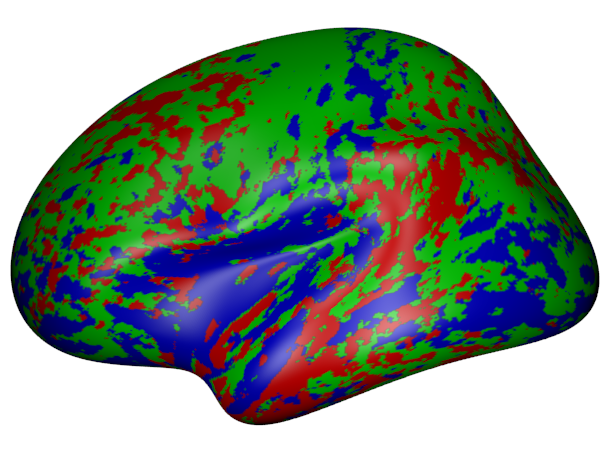
\includegraphics[width=\scalingFactorBrains\textwidth, trim=270 190 40 70, clip]{figures/blend14_adniThavgFWHM0InithistCl3Pr0Ra1_VWDPMStd.png}}; 
    \node[inner sep=0] (label) at (0,3.5) {tAD - ADNI};
  \end{tikzpicture}
%     \caption{}
%       \label{fig:adniClust}
  \end{subfigure}
   \begin{subfigure}[b]{0.3\textwidth}
  \centering
  \begin{tikzpicture}[scale=\scalingFactor, every node/.style={scale=\scalingFactor}]
    \node[inner sep=0] (corr_text) at (0,0) {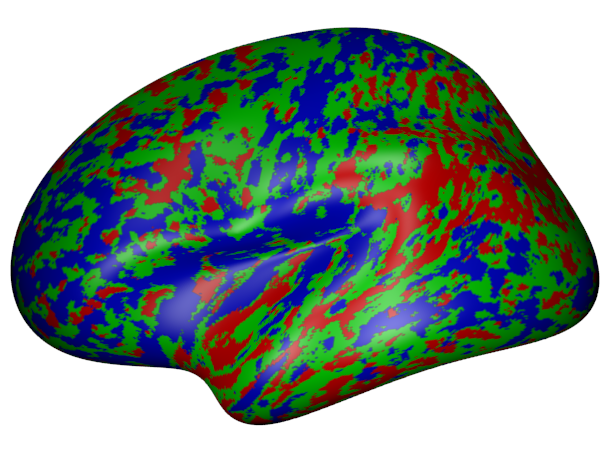
\includegraphics[width=\scalingFactorBrains\textwidth, trim=270 190 40 70, clip]{figures/drcThavgFWHM0InithistCl3Pr0Ra1_VWDPMStdAD_blend24.png}};
    \node[inner sep=0] (label) at (0,3.5) {tAD - UCL DRC dataset};
  \end{tikzpicture}
%     \caption{}
%       \label{fig:drcClustAD}
  \end{subfigure}
   \begin{subfigure}[b]{0.3\textwidth}
  \centering
  \begin{tikzpicture}[scale=\scalingFactor, every node/.style={scale=\scalingFactor}]
    \node[inner sep=0] (corr_text) at (0,0) {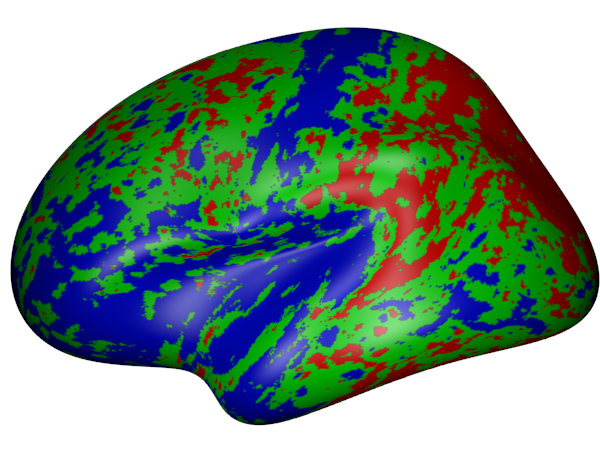
\includegraphics[width=\scalingFactorBrains\textwidth, trim=270 190 40 70, clip]{figures/drcThavgFWHM0InithistCl3Pr0Ra1_VWDPMStdPCA_blend24.png}};
    \node[inner sep=0] (label) at (0,3.5) {PCA - UCL DRC dataset};
  \end{tikzpicture}
%     \caption{}
%       \label{fig:drcClustPCA}
  \end{subfigure}
  
  %%%%%%%%%%%%%%%%%%%%%% trajectories %%%%%%%%%%%%%%%%%%%%%%%
  
    \begin{subfigure}[b]{0.3\textwidth}
    \centering
%     \vspace{-2em}
    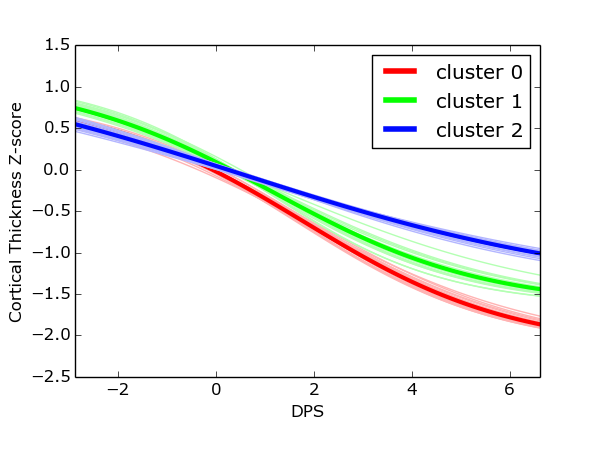
\includegraphics[width=\scalingFactor\textwidth]{figures/trajSamplesOneFig_adniThavgFWHM0InithistCl3Pr0Ra1_VWDPMStd.png}
%     \caption{}
%       \label{fig:adniTraj}
  \end{subfigure}
      \begin{subfigure}[b]{0.3\textwidth}
    \centering
%     \vspace{-2em}
    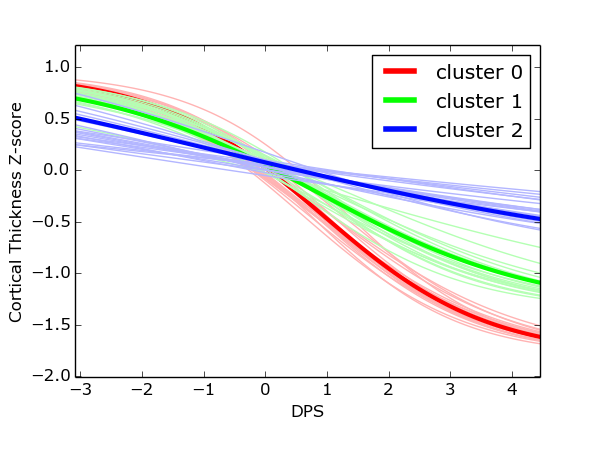
\includegraphics[width=\scalingFactor\textwidth]{figures/trajSamplesOneFig_drcThavgFWHM0InithistCl3Pr0Ra1_VWDPMStdAD.png}
%     \caption{}
%       \label{fig:drcTrajAD}
  \end{subfigure}
    \begin{subfigure}[b]{0.3\textwidth}
    \centering
%     \vspace{-2em}
    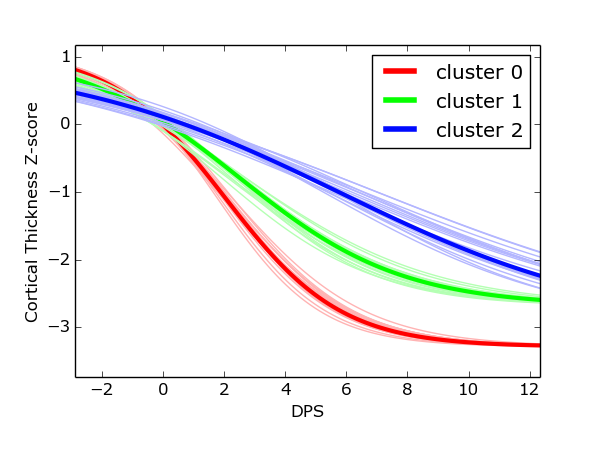
\includegraphics[width=\scalingFactor\textwidth]{figures/trajSamplesOneFig_drcThavgFWHM0InithistCl3Pr0Ra1_VWDPMStdPCA.png}
%     \caption{}
%       \label{fig:drcTrajPCA}
  \end{subfigure}
  
%   \caption{}
%   \label{fig:clustTrajAll}

\end{figure}

\vspace{-1em}

\textbf{Conclusions:}
\begin{itemize}
 \item Similar patterns of atrophy in tAD in two independent datasets: ADNI and UCL DRC
 \item Distinct patterns of atrophy in two different diseases: typical AD and Posterior Cortical Atrophy
\end{itemize}


\end{frame}


%%%%%%%%%%%%%%%%%%%%%%%%%%%%%%%%%%%%%%%%%%%%%%%%%%%%%%%%%%%%%5

\begin{frame}
\frametitle{Results - ADNI and UCL DRC Cohorts}
%% slide 4 - comparison with previous literature

\newcommand{\scalingFactor}{0.8}

\newcommand{\gradLimLeft}{-1.6}
\newcommand{\gradLimRight}{1.6}

% \newcommand{\scalingFactorLeftFig}{1.2}
\newcommand{\scalingFactorBrains}{1}
\newcommand{\scalingFactorTraj}{1}

\textbf{Results resemble previous findings in the literature}

\vspace{0.5em}
% FWHM0 avg thickness map MCI & AD
\begin{figure}[h]
  \centering
  % do the legend colorbar
  \begin{subfigure}[b]{\textwidth}
   \centering
  \begin{tikzpicture}[scale=1.9*\scalingFactor, every node/.style={scale=0.8*\scalingFactor}]
    \shade[left color=red,right color=green] (\gradLimLeft,2.5) rectangle (0,2.75);
    \shade[left color=green,right color=blue] (0,2.5) rectangle (\gradLimRight,2.75);
    \node[inner sep=0] (corr_text) at (\gradLimLeft,2.25) {cluster 0};
    \node[inner sep=0] (corr_text) at (0,2.25) {cluster 1};
    \node[inner sep=0] (corr_text) at (\gradLimRight,2.25) {cluster 2};
    \node[inner sep=0] (corr_text) at (\gradLimLeft,3) {rapid atrophy};
    \node[inner sep=0] (corr_text) at (\gradLimRight,3) {slow atrophy};
  \end{tikzpicture}
%     \caption{}
%       \label{fig:adniClust}
  \vspace{1em}
  \end{subfigure}
  
  %%%%%%%%%%%%%%%%%%% BRAINS %%%%%%%%%%%%%%5%%%%%%
  
  %%%%%%%% slide 4 %%%%%%%%%%%%%
  
  \begin{subfigure}[b]{0.3\textwidth}
   \centering
  \begin{tikzpicture}[scale=\scalingFactor, every node/.style={scale=\scalingFactor}]
    \node[inner sep=0] (image) at (0,0) {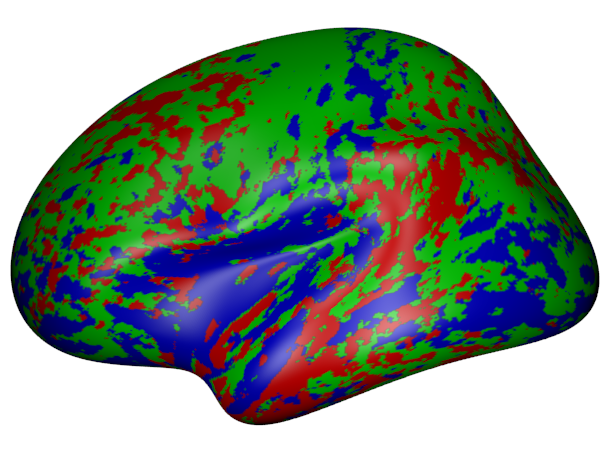
\includegraphics[width=\scalingFactorBrains\textwidth]{figures/blend14_adniThavgFWHM0InithistCl3Pr0Ra1_VWDPMStd.png}}; 
    \node[inner sep=0] (label) at (0,3.5) {tAD - ADNI};
  \end{tikzpicture}
%     \caption{}
%       \label{fig:adniClust}
  \end{subfigure}
   \begin{subfigure}[b]{0.3\textwidth}
  \centering
  \begin{tikzpicture}[scale=\scalingFactor, every node/.style={scale=\scalingFactor}]
    \node[inner sep=0] (corr_text) at (0,0) {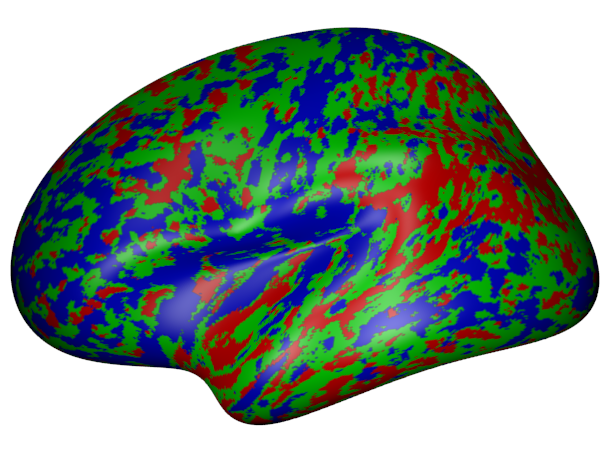
\includegraphics[width=\scalingFactorBrains\textwidth]{figures/drcThavgFWHM0InithistCl3Pr0Ra1_VWDPMStdAD_blend24.png}};
    \node[inner sep=0] (label) at (0,3.5) {tAD - UCL DRC dataset};
  \end{tikzpicture}
%     \caption{}
%       \label{fig:drcClustAD}
  \end{subfigure}
   \begin{subfigure}[b]{0.3\textwidth}
  \centering
  \begin{tikzpicture}[scale=\scalingFactor, every node/.style={scale=\scalingFactor}]
    \node[inner sep=0] (corr_text) at (0,0) {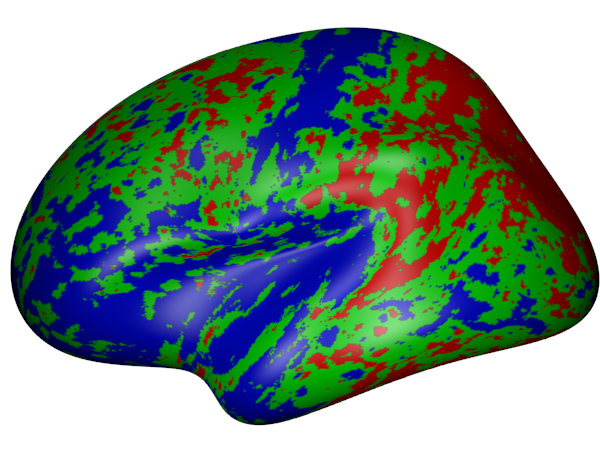
\includegraphics[width=\scalingFactorBrains\textwidth]{figures/drcThavgFWHM0InithistCl3Pr0Ra1_VWDPMStdPCA_blend24.png}};
    \node[inner sep=0] (label) at (0,3.5) {PCA - UCL DRC dataset};
  \end{tikzpicture}
%     \caption{}
%       \label{fig:drcClustPCA}
  \end{subfigure}
%   \vspace{1em}

  \begin{subfigure}[b]{0.65\textwidth}
  \centering
  \vspace{1em}
  tAD Cortical Thinning\\ \small{Dickerson et al., Cereb. Cortex, 2009}
  
  \includegraphics[width=0.35\textwidth]{dickerson_ad_lateral.png}
  \end{subfigure}
  \hspace{-1em}
  \begin{subfigure}[b]{0.3\textwidth}
  \centering
  \vspace{1em}
  
  PCA Cortical Thinning\\ \small{Lehmann et al., Neurobiol. of Aging, 2011}

  \includegraphics[width=0.65\textwidth]{lehmann_2011_brain}
  \end{subfigure}
    
\end{figure}
\vspace{-2em}

\end{frame}





%%%%%%%%%%%%%%%%%%%%%%%%%%%%%%%%%%%%%%%%%%%%%%%%%%%%%%%%%%%%%5

\newcommand{\ipmiPaperFold}{../}
\newcommand{\outFoldADNICVbrains}{\ipmiPaperFold/figures/crossvalid/adniThavgFWHM0Initk-meansCl3Pr0Ra1_VWDPMMean}
\newcommand{\scaleFig}{0.16}

\begin{frame}
\frametitle{Results - Validation of Estimated Atrophy Patterns}

\textbf{Cross-validation}
\begin{itemize}
 \item Tested the consistency of the spatial clustering in ADNI using 10-fold CV
 \item Results show good agreement in terms of spatial distribution
 \item Average dice score overlap for all cluster pairs: 0.89
\end{itemize}


\begin{figure}[h]
    \centering
    
%     \newcounter{classnumber}
    \foreach \n in {0,...,9}{
    \begin{subfigure}[b]{\scaleFig\textwidth}
    \includegraphics[width=\textwidth]{\outFoldADNICVbrains/blend\n.png}\\
    \vspace{-1.5em}
    \includegraphics[width=\textwidth,trim=0 0 0 25,clip]{figures/cogCorr/trajSamplesOneFig_cogCorr_adniThFWHM0Initk-meansCl3Pr0Ra1Mrf5_VWDPMMean_f\n.png}
    \end{subfigure}
    }
    
%     \caption{Cross-validation}
    \label{fig:ADNICVbrains}
\end{figure}

\end{frame}

%%%%%%%%%%%%%%%%%%%%%%%%%%%%%%%%%%%%%%%%%%%%%%%%%%%%%%%%%%%%%

\begin{frame}
\frametitle{Results - Validation of Estimated Subject Progression Scores}

\textbf{Hypotheses}: 
\begin{enumerate}
 \item Subjects show higher disease progression \\score (DPS) in later visits
 \item DPS correlates with other markers of \\disease progression
\end{enumerate}

\vfill

\textbf{Method}: Ran our model on ADNI using \\10-fold cross-validation

\vfill

\textbf{Results}
\begin{enumerate}
 \item 84\% of subjects analysed show increasing DPS 
 \item Progression scores correlate well with cognitive tests:
\end{enumerate}

\vspace{-16em}
\begin{figure}[h]
%   \right
  \includegraphics[width=0.4\textwidth,right]{\ipmiPaperFold/figures/crossvalid/stagingConsist_adniThavgFWHM0Initk-meansCl3Pr0Ra1_VWDPMMean.png}
\end{figure}

% \vspace{2em}


\newcommand{\figFont}{\small}
\newcommand{\pValFont}{\tiny}

\begin{figure}[h]
  \begin{subfigure}{0.22\textwidth}
    \centering
    \figFont{CDRSOB}\\ \pValFont{($\rho = 0.41$, $p < 1e-66$)}
    \includegraphics[width=1.1\textwidth]{figures/stagingCogTestsScatterPlot_adniThFWHM0Initk-meansCl3Pr0Ra1Mrf5_VWDPMMean_ADAS13.png}
  \end{subfigure}
  \begin{subfigure}{0.22\textwidth}
    \centering
    \figFont{ADAS-COG}\\ \pValFont{($\rho = -0.40$, $p < 1e-62$)}
    \includegraphics[width=1.1\textwidth]{figures/stagingCogTestsScatterPlot_adniThFWHM0Initk-meansCl3Pr0Ra1Mrf5_VWDPMMean_MMSE.png}
  \end{subfigure}
    \begin{subfigure}{0.22\textwidth}
    \centering
    \figFont{MMSE}\\ \pValFont{($\rho = -0.39$, $p < 1e-58$)}
    \includegraphics[width=1.1\textwidth]{figures/stagingCogTestsScatterPlot_adniThFWHM0Initk-meansCl3Pr0Ra1Mrf5_VWDPMMean_RAVLT.png}
  \end{subfigure}
    \begin{subfigure}{0.22\textwidth}
    \centering
    \figFont{RAVLT}\\ \pValFont{($\rho = 0.39$, $p < 1e-58$)}
    \includegraphics[width=1.1\textwidth]{figures/stagingCogTestsScatterPlot_adniThFWHM0Initk-meansCl3Pr0Ra1Mrf5_VWDPMMean_CDRSOB.png}
  \end{subfigure}
\end{figure}

% \vspace{-4em}


\end{frame}


%%%%%%%%%%%%%%%%%%%%%%%%%%%%%%%%%%%%%%%%%%%%%%%%%%%%%%%%%%%%%%%%%



\begin{frame}
\frametitle{Recent Work - Results on PET imaging}

\newcommand{\scalingFactor}{1}

\newcommand{\gradLimLeft}{-1.6}
\newcommand{\gradLimRight}{1.6}

% \newcommand{\scalingFactorLeftFig}{1.2}
\newcommand{\scalingFactorBrains}{1.0}
\newcommand{\scalingFactorTraj}{1}

\newcommand{\recentFigFold}{../../journal_paper/figures/}

\begin{columns}[T]
%     \hspace{-4em}
    \begin{column}{.55\textwidth}
    
    \vspace{3em}
    \textbf{Motivation}
    \begin{itemize}
      \item Prove the model can be used on other types of data
      \item Hypothesis: PET clusters will be different from cortical thickness ones
    \end{itemize}
    
%     \vspace{2em}
    
    \textbf{Methods}
    \begin{itemize}
      \item Used 433 subjects from ADNI with PET AV45 scans
      \item Preprocessing with the PETSurfer pipeline
    \end{itemize}
    
%     \vspace{2em}
    
    \textbf{Conclusion}
    \begin{itemize}
      \item PET deposition patterns are focused on precuneus and frontal areas
     \item Spatial patterns match with previous findings (Bilgel et al., IPMI, 2015)
     \item Model still works with PET data, which is more spatially correlated
    \end{itemize}
     
    \end{column}
    
    \begin{column}{.4\textwidth}
      \begin{figure}[h]
	\centering
	Our model
	% TODO: fix colorbar colours, interpolate through yellow and cyan
	% do the legend colorbar
	\begin{subfigure}[b]{\textwidth}
	\centering
	\vspace{1em}
	\begin{tikzpicture}[scale=1.9*\scalingFactor, every node/.style={scale=0.8*\scalingFactor}]
	  \shade[left color=red,right color=green] (\gradLimLeft,2.5) rectangle (0,2.75);
	  \shade[left color=green,right color=blue] (0,2.5) rectangle (\gradLimRight,2.75);
      %     \node[inner sep=0] (corr_text) at (\gradLimLeft,2.25) {cluster 0};
      %     \node[inner sep=0] (corr_text) at (0,2.25) {cluster 1};
      %     \node[inner sep=0] (corr_text) at (\gradLimRight,2.25) {cluster 2};
	  \node[inner sep=0] (corr_text) at (\gradLimLeft,3) {rapid atrophy};
	  \node[inner sep=0] (corr_text) at (\gradLimRight,3) {slow atrophy};
	\end{tikzpicture}
      %     \caption{}
      %       \label{fig:adniClust}
% 	\vspace{1em}
	\end{subfigure}
	
	%%%%%%%%%%%%%%%%%%% BRAINS %%%%%%%%%%%%%%%%%%%%
	
	  \begin{subfigure}[b]{0.6\textwidth}
	\centering
	\begin{tikzpicture}[scale=\scalingFactor, every node/.style={scale=\scalingFactor}]
	  \node[inner sep=0] (corr_text) at (0,0) {\includegraphics[width=\scalingFactorBrains\textwidth]{\recentFigFold/slopeCol_adniPetInitk-meansCl20Pr0Ra1Mrf5DataNZ_VDPM_MRF.png}};
% 	  \node[inner sep=0] (label) at (0,3.5) {ADNI AV45 PET};
	\end{tikzpicture}
      %     \caption{}
      %       \label{fig:drcClustPCA}
	\end{subfigure}
	
	%%%%%%%%%%%%%%%%%%%%%% trajectories %%%%%%%%%%%%%%%%%%%%%%%

	
      \begin{subfigure}[b]{0.8\textwidth}
      \hspace{-1em}
	\begin{tikzpicture}[width=\textwidth]
	\node[inner sep=0] (corr_text) at (0,0){\includegraphics[width=\scalingFactor\textwidth,trim=30 0 0 83,clip]{\recentFigFold/trajSamplesOneFig_adniPetInitk-meansCl20Pr0Ra1Mrf5DataNZ_VDPM_MRF.png}};
	\node[rotate=90] (ylabel) at (-5.2,0.7) {\tiny{-SUVR}};
	\end{tikzpicture}
      \end{subfigure}
      
      \begin{subfigure}[b]{0.8\textwidth}
      \centering
      \vspace{1em}
      Bilgel et al, IPMI, 2015
      \includegraphics[width=0.6\textwidth,trim=210 0 140 0,clip]{bilgel_neuroimage}
      \end{subfigure}
      
      
      \end{figure}
    \end{column}
  \end{columns}

\end{frame}

\begin{frame}
\frametitle{Summary}

% \textbf{Summary}:
Developed a method that:
\begin{itemize}
\item finds disconnected regions which undergo similar disease progression dynamics
\item simultaneously estimates biomarker trajectories
\item completely new way of parcellating the brain based on disease progression
\item applicable to any kind of vertexwise/voxelwise data (e.g. MRI, PET, DTI)
\end{itemize}

% \vfill

% Model features:
% \begin{itemize}
% \item applicable to any kind of vertexwise/voxelwise data
% \item easily extensible (e.g. MRF)
% \end{itemize}

\vfill

Findings:
\begin{itemize}
\item Model finds plausible patterns in four different datasets
\item Estimated disease progression scores are clinically relevant
\end{itemize}

 % Validation
 % model was 
 
\end{frame}

\begin{frame}
\frametitle{Limitations and Future Work}

% \begin{tabular}{p{4cm} p{4cm}}
%  \textbf{Limitations} & \textbf{Future work} \\
%  The model assumes all patients follow the same progression pattern & Model distinct progression patterns for distinct subgroups\\
%  Biomarker trajectories are assumed sigmoidal & Model is easily extensible to non-parametric shapes\\
%  Model relies on a well-defined control population & Define control population using data-driven techniques (e.g. mixture models)\\
% \end{tabular}

\begin{columns}[T]
%     \hspace{-4em}
    \begin{column}{.45\textwidth}
    \textbf{Limitations}
    \begin{enumerate}
     \item The model assumes all patients follow the same progression pattern \break
     \item Biomarker trajectories are assumed sigmoidal
     \item Model relies on a well-defined control population \break
     \item Model doesn't allow variability in cluster trajectories
    \end{enumerate}
    \end{column}
    
    \begin{column}{.45\textwidth}
    \textbf{Future work}
    \begin{enumerate}
     \item Model distinct progression patterns for population subgroups (e.g. Young et al., IPMI, 2015)
     \item Our model is easily extensible to non-parametric trajectories
     \item Define control population using data-driven techniques (e.g. mixture models).
     \item Fit parameters using variational methods (e.g. Variational Bayes)
    \end{enumerate}
    
    \end{column}
  \end{columns}
  
  \vspace{2em}
  
\textbf{Work in progress}:
\begin{itemize}
 \item Correlate the cluster patterns with a structural connectome from the HCP dataset
 \item Hypothesis: disconnected areas cluster together due to underlying WM connections
\end{itemize}


\end{frame}

\begin{frame}
\frametitle{Acknowledgements}

\includegraphics[width=\textwidth,trim=0 0 0 150, clip]{cmic_away_day}
 
 \begin{small}
\begin{columns}[T]
%     \hspace{-4em}
    \begin{column}{.45\textwidth}
    \textbf{Collaborators}
    \begin{enumerate}
     \item Leon Aksman
     \item Maura Bellio
     \item Arman Eshaghi
     \item Nicholas Firth
     \item Sara Garbarino
     \item Kyriaki Mengoudi 
     \item Marco Lorenzi
     \item Neil Oxtoby
     \item Peter Wijeratne
     \item Alexandra Young
    \end{enumerate}
%     \includegraphics[scale=1]{pondLogo.png}  
    \end{column}
    
    
    \begin{column}{.45\textwidth}
    \begin{center}
    \textbf{Project supervisors}
    \end{center}
    \vspace{-2em}
      \begin{figure}
      \begin{subfigure}{0.45\textwidth}
      \centering
      Daniel Alexander
      \includegraphics[scale=0.25]{Danny-Alexander.jpeg}  
      \end{subfigure}
	\begin{subfigure}{0.45\textwidth}
	\centering
	Sebastian Crutch
      \includegraphics[scale=0.27]{Seb_Crutch_photo.JPG}  
      \end{subfigure}
      
      \vspace{2em}

	\textbf{Funders}\\
	\vspace{1em}
% 	\begin{subfigure}{0.3\textwidth}
% 	\centering
	\includegraphics[height=1.0cm]{CDTlogo.png} \hspace{1em} \includegraphics[height=1.0cm]{epsrc_logo.jpg}
% 	\vspace{1em}	
% 	\end{subfigure}

\end{figure}
    
\end{column}
\end{columns}
 
\end{small}


\end{frame}


\begin{frame}
\frametitle{Join the TADPOLE challenge!}

\begin{itemize}
 \item Challenge: use any model of choice to predict future AD biomarkers
 \item URL: https://tadpole.grand-challenge.org/
 \item See me for flyers or more details!
\end{itemize}

\begin{figure}
\centering
\includegraphics[scale=0.4,trim=0 270 0 0,clip]{tadpole} 
\end{figure}


\end{frame}


%%%% END OF MAIN PRESENTATION %%%

%%%%%%%%%%%%%%%%%%%%%%%%%%%%%%%%%%%%%%%%%%%%%%%%%%%%%%%%%%%%%%%%%


\begin{frame}
\frametitle{Results - Comparison with Other Models}


\textbf{Hypotheses}
\begin{itemize}
 \item Dynamic clustering improves staging and biomarker prediction
 \item Subject staging improves biomarker prediction
\end{itemize}

\vfill

\textbf{Methods}
Compared the performance of our model to two simplified models:
 \begin{enumerate}
  \item Predefined ROI model (i.e. Jedynak et al., Neuroimage, 2012)
  \item Dynamic clustering only model, without subject staging: fixes $\alpha_i=1$, $\beta_i=0$, $\forall i$
 \end{enumerate}

\vfill
 
\textbf{Results}
\begin{itemize}
 \item Correlation $\rho$ between progression scores and cognitive tests
 \item Cortical thickness prediction error (RMSE)
\end{itemize}
\setlength\tabcolsep{0.1cm}
\begin{figure}
\begin{subfigure}{1\textwidth}
\centering
\begin{table}
\begin{footnotesize}
 \begin{tabular}{c | c c c c | c}
  Model & CDRSOB ($\rho$) & ADAS13 ($\rho$) & MMSE ($\rho$) & RAVLT ($\rho$) & Prediction (RMSE)\\
  \hline 
  Dynamic clusters + staging (our model) & 0.35 & 0.36 & 0.35 & 0.31 & 1.007 +/- 0.011\\
  Predefined ROI (Jedynak et al., Nimg, 2012) & 0.39 & 0.40 & 0.40 & 0.34 & 1.008 +/- 0.012\\
  Dynamic clusters, no staging & *0.02 & *-0.02 & *-0.02 & *0.01 & *1.058 +/- 0.021\\
 \end{tabular}
 \end{footnotesize}
\end{table}
% \caption{Mean correlation $\rho$ across all folds.}
\end{subfigure}
% \begin{subfigure}{0.45\textwidth}
% \centering
% \small{Prediction of future \\ biomarker values (RMSE)}
% \begin{table}
% \begin{tiny}
% \begin{tabular}{c | c c c c}
%   Model & ADNI - Thickness\\
%   \hline 
%   Dynamic clusters + staging (our model) &  1.007 +/- 0.011 \\
%   Static ROI & 1.008 +/- 0.012\\
%   Dynamic clusters, no staging & *1.058 +/- 0.021\\
% \end{tabular}
% \end{tiny}
% \end{table}
% \caption{RMSE values, mean $+/-$ std.}
% \end{subfigure}
\end{figure}



\textbf{Conclusion}
\begin{itemize}
 \item Dynamic clustering doesn't improve performance vs Predefined ROI model
 \item Disease staging of subjects improves performance vs model without staging
\end{itemize}


% \end{itemize}

\end{frame}



\section{Recent Work}

\begin{frame}
\frametitle{Recent Work - Modelling Spatial Correlation}

\textbf{Motivation}
\begin{itemize}
 \item measurements from neighouring vertices are inherently correlated
 \item could enable better staging and prediction
\end{itemize}


% MRF extension
\textbf{Method}:
\begin{itemize}
 \item Original formulation assumes independence between vertices
 \item Modelled spatial correlation between vertices with a \emph{Markov Random Field} (MRF):
$$ p(V, Z | \alpha, \beta, \theta, \sigma) = \prod_l^L \prod_{(i,j) \in I} N(V_l^{ij} | f(\alpha_i t_{ij} + \beta_i | \theta_{Z_l}), \sigma_{Z_l}) \textcolor{red}{\prod_{l_1 \sim l_2} \Psi (Z_{l_1}, Z_{l_2})}$$

% where 
% \begin{itemize}
%  \item $
%  \Psi (Z_{l_1}=k_1, Z_{l_2}=k_2) = 
%  \begin{cases}
%   exp(\alpha) & \text{if } k_1 = k_2\\
%   exp(-\alpha) & \text{otherwise}
%  \end{cases}
% $
%  \item $\alpha$ - MRF parameter
% \end{itemize}


\vspace{-1em}

\begin{figure}
\begin{subfigure}{0.3\textwidth}
\centering
 \includegraphics[scale=0.15]{slopeCol_drcThFWHM0Initk-meansCl3Pr0Ra1Mrf5_VWDPMMeanAD.png}
 \caption{Without MRF}
 \end{subfigure}
 \begin{subfigure}{0.3\textwidth}
 \centering
 \includegraphics[scale=0.15]{slopeCol_drcThFWHM0Initk-meansCl3Pr0Ra1Mrf5_VDPM_MRFAD.png}
 \caption{With MRF,  $\alpha = 5$.}
 \end{subfigure}
\end{figure}

  \item Work still in progress (not included in paper)

\end{itemize}

\end{frame}



% \begin{frame}
% \frametitle{Extra - BIC analysis}
% 
% \begin{itemize}
%  \item ADNI Cortical thickness:
%  \begin{itemize}
%   \item BIC: 2 clusters
%   \item AIC: 6 clusters
%  \end{itemize}
% \end{itemize}
% 
% \begin{figure}
% \centering
% \includegraphics[scale=0.4]{BICres_adniThFWHM0Initk-meansPr0Ra1Mrf5.png}
% \end{figure}
% 
% \end{frame}


\end{document}



